%=======================================================================
% cap3_bases_teoricas.tex — Bases teóricas
%=======================================================================

Este capítulo plantea las preguntas de investigación y los objetivos sobre
la brecha identificada en el \capref{cap:relacionado} y presenta, desde la
base, los fundamentos de los métodos que usa el sistema: cómo clasifica y
cómo se entrena una red neuronal, qué son una red convolucional y un
\textit{transformer}, cómo se convierte un sonido en una imagen que esas
redes pueden leer, cómo se combinan dos modalidades, cómo se modela la
distribución de una especie a partir de registros de solo presencia y cómo
se evalúa todo lo anterior. Cierra con la metodología de trabajo, las
fuentes de datos y los \textit{baselines}, y con la justificación técnica de
las decisiones tomadas.

%-----------------------------------------------------------------------
\section{Preguntas de investigación, objetivo general y objetivos específicos}
\label{sec:objetivos}

\subsection*{Preguntas de investigación}

\begin{enumerate}[label=\textbf{PI\arabic*.}, leftmargin=*, itemsep=3pt]
  \item ¿Puede un sistema de aprendizaje profundo multimodal identificar
        especies de aves chilenas a partir de audio y/o imagen con mejor
        desempeño que los clasificadores unimodales (solo audio o solo
        imagen) y que un modelo de IA generativa multimodal?
  \item ¿Puede un modelo de distribución de especies basado en aprendizaje
        automático (redes neuronales, Random Forest o gradient boosting), que integra
        avistamientos de ciencia ciudadana, clima e índices de vegetación
        satelitales, superar a MaxEnt bajo un protocolo de validación
        espacial?
  \item ¿Cómo afecta la escasez de datos de las especies amenazadas al
        desempeño de estos modelos? ¿Qué estrategias de aumentación y
        balanceo mitigan ese efecto?
\end{enumerate}

\subsection*{Objetivo general}

Desarrollar y evaluar un sistema de monitoreo de biodiversidad aviar que
integre la identificación multimodal (audio e imagen) y el modelado de
distribución espaciotemporal para especies de aves de Chile continental, con
foco en especies endémicas y amenazadas.

\subsection*{Objetivos específicos}

\begin{enumerate}[label=\textbf{OE\arabic*.}, leftmargin=*, itemsep=3pt]
  \item Construir un conjunto de datos curado y reproducible a partir de
        fuentes heterogéneas (Xeno-canto, iNaturalist/GBIF, registros de
        avistamientos, covariables ambientales satelitales y climáticas vía
        Google Earth Engine y el RCE del MMA), con particiones libres de fuga
        de información.
  \item Entrenar y evaluar clasificadores de audio (CNN/AST) e imagen
        (EfficientNet), e integrarlos mediante \textit{late fusion},
        alcanzando una \textit{accuracy} superior al \SI{85}{\percent} en al
        menos 50 especies.
  \item Entrenar modelos de distribución espaciotemporal basados en
        aprendizaje automático (redes neuronales, Random Forest y gradient boosting) y
        compararlos con un \textit{baseline} MaxEnt, incluida la validación
        cruzada espacial por bloques.
  \item Comparar el clasificador propuesto con un modelo de IA generativa
        multimodal mediante \textit{prompting} (\textit{zero-shot} y
        \textit{few-shot}), para situar su desempeño frente a una herramienta
        de uso general.
  \item Documentar el desempeño (\textit{accuracy}, F1 macro, AUC-ROC, tiempos
        de entrenamiento e inferencia) y las limitaciones, en particular el
        efecto de la escasez de datos en las especies amenazadas.
\end{enumerate}

La meta del \SI{85}{\percent} de \textit{accuracy} del OE2 se fijó en la
propuesta del proyecto como un nivel exigente pero alcanzable para un
problema \textit{fine-grained} de más de cincuenta clases con pocos datos
por especie. Es el nivel a partir del cual un asistente de identificación
acierta en más de cinco de cada seis consultas, lo que lo vuelve útil como
apoyo a un observador. Queda muy por encima de lo que logra el clasificador
global de referencia en Sudamérica (BirdNET, con \textit{recall} entre 0,24
y 0,52 según el continente, \tabref{tab:birdnet}) y es comparable al que
alcanzan los clasificadores regionales entrenados con conjuntos de datos
mucho mayores. Un umbral más bajo no serviría como herramienta de apoyo, y uno
más alto no sería realista con pocas decenas de grabaciones por especie.

%-----------------------------------------------------------------------
\section{Clasificación supervisada con redes neuronales}\label{sec:teoria-redes}

\subsection{El problema de clasificación y la salida softmax}

Clasificar es asignar una entrada $\mathbf{x}$ (una ventana de audio, una
fotografía) a una de $K$ clases disjuntas $\mathcal{C}_1, \dots,
\mathcal{C}_K$, aquí las $K = 55$ especies objetivo. Un clasificador útil no
solo decide: entrega, para cada clase, una probabilidad posterior
$p(\mathcal{C}_k \mid \mathbf{x})$ que expresa cuánta evidencia hay a favor
de esa especie. Separar la estimación de probabilidades de la decisión
final permite rechazar casos dudosos, compensar clases desbalanceadas y
combinar las salidas de varios modelos, que es justamente lo que hará la
fusión multimodal. La regla que
minimiza el número de errores es elegir la clase de mayor probabilidad
posterior \citep[pp.~140--147]{bishop2024deep}:
\begin{equation}
  \hat{y} = \argmax_{k \in \{1,\dots,K\}} \; p(\mathcal{C}_k \mid \mathbf{x}).
  \label{eq:argmax}
\end{equation}

Una red neuronal produce para cada clase un puntaje real $a_k$
(\textit{logit}) y convierte esos puntajes en probabilidades con la función
\textit{softmax}, llamada así porque es una versión suavizada del máximo: si
un puntaje domina a los demás, su probabilidad tiende a uno
\citep[p.~152]{bishop2024deep}:
\begin{equation}
  p(\mathcal{C}_k \mid \mathbf{x}) = y_k = \frac{\exp(a_k)}{\sum_{j=1}^{K} \exp(a_j)},
  \qquad 0 \le y_k \le 1, \quad \sum_{k=1}^{K} y_k = 1.
  \label{eq:softmax}
\end{equation}

\subsection{Verosimilitud y entropía cruzada}

Para entrenar la red hace falta una medida de cuán lejos están sus
probabilidades de las etiquetas verdaderas. Cada etiqueta se codifica como
un vector $\mathbf{t}_n$ con un uno en la clase correcta y ceros en el resto
(codificación 1-de-$K$). La
verosimilitud de las $N$ etiquetas de entrenamiento es el producto de las
probabilidades que la red asigna a las clases correctas, $\prod_n \prod_k
y_{nk}^{t_{nk}}$. Maximizarla equivale a minimizar su logaritmo negativo, la
\emph{entropía cruzada} \citep[p.~162]{bishop2024deep}:
\begin{equation}
  E(\mathbf{w}) = -\sum_{n=1}^{N} \sum_{k=1}^{K} t_{nk} \ln y_k(\mathbf{x}_n, \mathbf{w}),
  \label{eq:ce}
\end{equation}
donde $\mathbf{w}$ reúne todos los parámetros de la red. La entropía cruzada
penaliza con fuerza las predicciones seguras y equivocadas (si $y_k \to 0$
para la clase correcta, $-\ln y_k \to \infty$) y su gradiente respecto de los
logits tiene la forma simple $y_k - t_k$, la diferencia entre la
probabilidad predicha y la etiqueta. Es la
pérdida con que se entrenan todos los clasificadores de esta tesis.

Cuando las clases tienen tamaños muy distintos, la red tiende a favorecer a
las mayoritarias. Una corrección habitual es ponderar la pérdida de cada
clase por un peso $\omega_k$ que decrece con su número de ejemplos $n_k$. La
pérdida balanceada por número efectivo de muestras usa $\omega_k \propto
(1-\beta)/(1-\beta^{n_k})$ \citep{cui2019classbalanced}. En el límite $\beta
\to 1$ el peso tiende a $1/n_k$, el inverso de la frecuencia, que es la
variante implementada aquí (normalizada para que los pesos promedien uno):
\begin{equation}
  E_{\mathrm{pond}}(\mathbf{w}) = -\sum_{n=1}^{N} \sum_{k=1}^{K} \omega_k\, t_{nk} \ln y_{nk},
  \qquad \omega_k = \frac{1/n_k}{\frac{1}{K}\sum_{j=1}^{K} 1/n_j}.
  \label{eq:ce-pond}
\end{equation}

\subsection{Redes neuronales y su entrenamiento}

Una red neuronal es una composición de transformaciones lineales y
funciones no lineales. En la forma más simple, el perceptrón multicapa, cada
capa $l$ calcula $\mathbf{z}^{(l)} = h\big(\mathbf{W}^{(l)} \mathbf{z}^{(l-1)}\big)$ a
partir de la salida de la capa anterior, con $\mathbf{z}^{(0)} = \mathbf{x}$ y
$\mathbf{W}^{(l)}$ una matriz de pesos aprendibles
\citep[pp.~181--187]{bishop2024deep}. La no linealidad $h$ es imprescindible: sin
ella toda la red colapsaría en un modelo lineal. La más usada es la unidad
lineal rectificada, $\mathrm{ReLU}(a) = \max(0, a)$, barata y libre del
problema de los gradientes que se desvanecen con la sigmoide. Con
suficientes unidades, una red de
dos capas puede aproximar cualquier función continua, pero el teorema solo
garantiza la existencia. En la práctica la profundidad permite representar
la misma función con muchos menos parámetros y aprender representaciones
jerárquicas, de rasgos simples a conceptos.

El entrenamiento minimiza la pérdida por \emph{descenso de gradiente}: en
cada paso los parámetros se mueven en la dirección contraria al gradiente,
$\mathbf{w}^{(\tau)} = \mathbf{w}^{(\tau-1)} - \eta \nabla E(\mathbf{w}^{(\tau-1)})$,
con una tasa de aprendizaje $\eta$. Como el
gradiente sobre todo el conjunto es costoso, se estima sobre minilotes de
$n_b$ ejemplos (descenso de gradiente estocástico). Una pasada completa por
los datos es una \emph{época}. El gradiente de cada parámetro se obtiene por
retropropagación. El optimizador Adam mantiene promedios móviles del
gradiente ($s_i$) y de su cuadrado ($r_i$) para adaptar el tamaño del paso a
cada parámetro \citep[pp.~222--224]{bishop2024deep}:
\begin{equation}
  w_i^{(\tau)} = w_i^{(\tau-1)} - \eta\, \frac{\hat{s}_i}{\sqrt{\hat{r}_i} + \delta},
  \label{eq:adam}
\end{equation}
con $\hat{s}_i$ y $\hat{r}_i$ corregidos por el sesgo de su inicialización en
cero y $\delta$ una constante pequeña de estabilidad. La variante AdamW,
usada en esta tesis, aplica el decaimiento de pesos de forma desacoplada del
gradiente \citep{loshchilov2019adamw}. La tasa de aprendizaje se reduce a
lo largo del entrenamiento (programación de coseno), porque conviene
empezar con pasos grandes y terminar con pasos finos.

%-----------------------------------------------------------------------
\section{Sobreajuste, regularización y aumentación de datos}\label{sec:teoria-regularizacion}

Una red con millones de parámetros puede memorizar el conjunto de
entrenamiento, incluido su ruido, y fallar con datos nuevos: es el
\emph{sobreajuste}. Se detecta comparando el error de entrenamiento con el de
un conjunto de validación: el primero baja siempre, mientras que el segundo
baja y luego sube cuando la red empieza a memorizar \citep[pp.~266--267]{bishop2024deep}.
La \emph{regularización} agrupa las técnicas que inducen a la red a preferir
soluciones más simples o más invariantes. La experiencia práctica se resume
en una regla: casi siempre generaliza mejor una red grande con
regularización que una red pequeña sin ella \citep[p.~254]{bishop2024deep}.
Las técnicas usadas en esta tesis son las siguientes.

\begin{itemize}[leftmargin=*, itemsep=2pt]
  \item \textbf{Decaimiento de pesos.} Se agrega a la pérdida un término
        $\frac{\lambda_{\mathrm{wd}}}{2}\mathbf{w}^{\mathrm{T}}\mathbf{w}$ que penaliza los pesos
        grandes. Su gradiente $\lambda_{\mathrm{wd}} \mathbf{w}$ empuja cada peso hacia cero
        salvo que los datos lo sostengan \citep[p.~260]{bishop2024deep}.
  \item \textbf{Parada temprana.} Se conserva el modelo de la época con mejor
        desempeño en validación, lo que limita cuánto puede ajustarse la red.
  \item \textbf{\textit{Dropout}.} Durante el entrenamiento se desactivan al
        azar unidades de la red. La red resultante es un promedio aproximado
        de muchas subredes y ninguna unidad puede depender de otra
        específica \citep[pp.~279--281]{bishop2024deep}.
  \item \textbf{Profundidad estocástica.} En redes con bloques residuales
        (\secref{sec:teoria-cnn}) se omiten bloques completos al azar, con
        probabilidad creciente hacia la salida. Acorta la red durante el
        entrenamiento y regulariza como el \textit{dropout}, pero a nivel de
        bloque \citep{huang2016stochasticdepth}.
  \item \textbf{Suavizado de etiquetas.} En vez de exigir probabilidad uno
        para la clase correcta, la etiqueta se reparte: $t_k = 1-\epsilon+\epsilon/K$
        para la clase correcta y $\epsilon/K$ para las demás (la variante
        que implementa PyTorch), con $\epsilon = 0{,}1$. Evita que la red se vuelva demasiado segura y
        mejora la calibración de sus probabilidades
        \citep{szegedy2016labelsmoothing}.
  \item \textbf{Aumentación de datos.} Se amplía el conjunto de entrenamiento
        con copias transformadas de cada ejemplo que conservan la etiqueta:
        recortes, volteos y cambios de color en imágenes, o ruido y cambios
        de ganancia en audio. Cada vez que el ejemplo se presenta se aplica
        una transformación distinta \citep[pp.~257--258]{bishop2024deep}.
        Es la forma más efectiva de enseñar invariancias cuando hay pocos
        datos.
  \item \textbf{\textit{Mixup}.} Se entrena con mezclas convexas de pares de
        ejemplos y de sus etiquetas \citep{zhang2018mixup}:
        \begin{equation}
          \tilde{\mathbf{x}} = \lambda \mathbf{x}_i + (1-\lambda)\mathbf{x}_j, \qquad
          \tilde{\mathbf{t}} = \lambda \mathbf{t}_i + (1-\lambda)\mathbf{t}_j, \qquad
          \lambda \sim \mathrm{Beta}(a, a),
          \label{eq:mixup}
        \end{equation}
        lo que obliga a la red a comportarse de forma suave entre ejemplos y
        reduce la memorización. Aquí $a = 0{,}2$.
  \item \textbf{SpecAugment.} Aumentación específica de espectrogramas: se
        enmascaran franjas aleatorias de frecuencia y de tiempo, de modo que
        la red no pueda apoyarse en una sola banda o en un solo instante del
        canto \citep{park2019specaugment}. La
        \figref{fig:representacion-audio} muestra un ejemplo de ambas
        aumentaciones de audio.
\end{itemize}

%-----------------------------------------------------------------------
\section{Redes convolucionales y EfficientNet}\label{sec:teoria-cnn}

\subsection{La operación de convolución}

Una fotografía (o un espectrograma) es una grilla de valores con fuerte
estructura local: dos píxeles vecinos suelen parecerse y un rasgo (un borde,
una mancha, un trino) ocupa una región pequeña y puede aparecer en cualquier
posición. Una red densa ignora esa estructura y necesitaría miles de
millones de pesos para una imagen de alta resolución. La red convolucional
(CNN) incorpora en su diseño la localidad, la jerarquía, la equivariancia y
la invariancia a traslaciones, y por eso necesita muchos menos datos
\citep[pp.~289--290]{bishop2024deep}. Su operación básica, la
\emph{convolución}, desliza un pequeño filtro o \textit{kernel} $\mathbf{U}$
de $s \times s$ pesos sobre toda la entrada $\mathbf{I}$ y calcula en cada
posición el producto punto entre el filtro y el parche que cubre
\citep[p.~292]{bishop2024deep}:
\begin{equation}
  C(p, q) = \sum_{l=1}^{s} \sum_{m=1}^{s} I(p+l,\, q+m)\, u_{lm} + b,
  \label{eq:conv}
\end{equation}
donde $C$ es el \emph{mapa de características}, $u_{lm}$ los pesos del
filtro y $b$ un sesgo. Cada filtro
actúa como un detector que se ``enciende'' (tras la ReLU) cuando el parche se
parece a su patrón. Como el mismo filtro recorre toda la imagen, un rasgo se
detecta esté donde esté, con muy pocos parámetros. Una capa aplica
$C_{\mathrm{out}}$ filtros distintos sobre los $C_{\mathrm{in}}$ canales de
entrada, con $(s^2 C_{\mathrm{in}} + 1)\,C_{\mathrm{out}}$ parámetros en
total. El \emph{pooling} resume bloques
vecinos con el máximo o el promedio: conserva si un rasgo está presente y
con qué fuerza, descarta parte de su posición exacta y reduce la
resolución, de modo que las capas siguientes ``ven'' regiones cada vez
mayores \citep[pp.~296--298]{bishop2024deep}. Apilando capas de convolución
y \textit{pooling}, los rasgos simples de las primeras capas (bordes, tonos
sostenidos) se combinan en patrones complejos (un pico, una sílaba del
canto) y, al final, un \textit{pooling} global y una capa densa con softmax
producen las $K$ probabilidades (\figref{fig:cnn}).

\begin{figure}[!htb]
  \centering
  \IfFileExists{figuras/tikz_cnn.tex}{\fitwidth{% Figura: red neuronal convolucional (tres paneles apilados).
% (a) operación de convolución, (b) arquitectura típica, (c) bloque residual.
% Unidades: 1 = 1 mm. Ancho total ~150 mm x alto ~125 mm (cabe en \textwidth = 160 mm).
\begin{tikzpicture}[x=1mm, y=1mm, font=\footnotesize,
  bloque/.style={draw, rounded corners, align=center, minimum height=8mm,
                 minimum width=20mm, font=\footnotesize, inner sep=1.5pt},
  dato/.style={bloque, fill=pucazul!15},
  capa/.style={bloque, fill=miaamarillo!30},
  proc/.style={bloque, fill=black!5},
  salida/.style={bloque, fill=green!12},
  flecha/.style={-{Latex[length=2mm]}, thick},
  flechita/.style={-{Latex[length=1.5mm]}, thin, pucgris},
  panel/.style={anchor=north west, font=\footnotesize\bfseries, inner sep=0pt},
  etq/.style={font=\footnotesize, align=center, inner sep=1pt},
  mini/.style={font=\scriptsize, align=center, inner sep=1pt}]

  % Pila de mapas de características: \pila{x}{lado}{n}{desplazamiento}{relleno}{nombre}
  \def\pila#1#2#3#4#5#6{%
    \foreach \k in {#3,...,1}{%
      \pgfmathsetmacro{\kk}{\k-1}%
      \draw[draw=pucgris, thin, rounded corners=0.4mm, fill=#5]
        ({#1+\kk*#4},{-#2/2+\kk*#4}) rectangle ++(#2,#2);}%
    \coordinate (#6w) at (#1,0);
    \coordinate (#6e) at ({#1+#2+min(#3-1,floor(#2/2/#4))*#4},0);}

  % ================= (a) Operación de convolución =================
  \begin{scope}[shift={(4,0)}]
    \node[panel] at (-4,36) {(a) Operación de convolución};
    % Entrada 6x6
    \begin{scope}[shift={(4,2)}]
      \foreach \i in {0,...,5} \foreach \j in {0,...,5}
        \fill[pucazul!15] (4*\i,4*\j) rectangle ++(4,4);
      % celdas "de señal" (coordenadas en mm; celda = 4 mm)
      \foreach \c in {(0,4),(4,4),(8,0),(16,8),(20,12),(20,16),(0,20),(12,20)}
        \fill[pucazul!40] \c rectangle ++(4,4);
      % ventana desplazada (punteada) debajo del relleno amarillo
      \draw[pucgris, thick, dashed] (8,8) rectangle (20,20);
      \fill[miaamarillo!50] (4,8) rectangle (16,20);
      \draw[pucgris!50, very thin] (0,0) grid[step=4] (24,24);
      \draw[pucgris, thick] (4,8) rectangle (16,20);
      \draw[flechita] (9,25.5) -- (15,25.5);
      \node[mini, anchor=south] at (12,26.3) {se desliza};
      \node[etq, anchor=north] at (12,-1) {Entrada\\(espectrograma o imagen)};
    \end{scope}
    % Filtro 3x3
    \draw[flecha] (28,14) -- (36,14) node[midway, above=0.3mm, mini] {$\ast$};
    \begin{scope}[shift={(36,8.75)}]
      \foreach \i in {0,1,2} \foreach \j in {0,1,2}
        \fill[miaamarillo!50] (3.5*\i,3.5*\j) rectangle ++(3.5,3.5);
      \draw[pucgris, very thin] (0,0) grid[step=3.5] (10.5,10.5);
      \draw[pucgris, thick] (0,0) rectangle (10.5,10.5);
      \node[etq, anchor=south] at (5.25,11.5) {Filtro $3{\times}3$};
      \node[mini, anchor=north] at (5.25,-1) {pesos $u_{l,m}$, sesgo $b$};
    \end{scope}
    % Mapa de características 4x4
    \draw[flecha] (46.5,14) -- (54.5,14);
    \begin{scope}[shift={(54.5,6)}]
      \foreach \i in {0,...,3} \foreach \j in {0,...,3}
        \fill[pucazul!15] (4*\i,4*\j) rectangle ++(4,4);
      \foreach \c in {(0,0),(12,4),(8,12)}
        \fill[pucazul!40] \c rectangle ++(4,4);
      \fill[miaamarillo!50] (4,8) rectangle (8,12);
      \draw[pucgris!50, very thin] (0,0) grid[step=4] (16,16);
      \draw[pucgris, thick] (4,8) rectangle (8,12);
      \node[etq, anchor=north] at (8,-1) {Mapa de\\características};
    \end{scope}
    % Fórmula
    \node[anchor=west, align=left, inner sep=0pt] at (75,14)
      {$\displaystyle C_{p,q} = \sum_{l,m} I_{p+l,\,q+m}\, u_{l,m} + b$\\[2mm]
       seguida de ReLU: $\max(0,\,C_{p,q})$};
  \end{scope}

  % ================= (b) Arquitectura típica =================
  \begin{scope}[shift={(0,-32)}]
    \node[panel] at (0,20) {(b) Arquitectura típica de una CNN para clasificación};
    % Entrada
    \draw[draw=pucgris, thin, rounded corners=0.4mm, fill=pucazul!15] (0,-6) rectangle (12,6);
    \node[mini, anchor=south] at (6,9.2) {$H\times W$};
    \node[etq, anchor=north] at (6,-6.8) {Entrada};
    % Bloques convolución + pooling (x3)
    \pila{18.5}{11}{3}{1.2}{miaamarillo!30}{c1}
    \pila{38.4}{8}{3}{1.2}{black!5}{p1}
    \pila{55.3}{8}{4}{1.1}{miaamarillo!30}{c2}
    \pila{73.1}{6}{4}{1.1}{black!5}{p2}
    \pila{88.9}{6}{5}{1.0}{miaamarillo!30}{c3}
    \pila{105.4}{4.5}{5}{1.0}{black!5}{p3}
    \node[etq, anchor=north] at (25.2,-6.8) {Convolución\\+ ReLU};
    \node[etq, anchor=north] at (60.95,-6.8) {Convolución\\+ ReLU};
    \node[etq, anchor=north] at (93.9,-6.8) {Convolución\\+ ReLU};
    \node[mini, anchor=south] at (25.2,9.2) {$C_1$ canales};
    \node[mini, anchor=south] at (60.95,9.2) {$C_2 > C_1$};
    \node[mini, anchor=south] at (93.9,9.2) {$C_3 > C_2$};
    \node[etq, anchor=south] at (43.6,9.2) {Pooling};
    \node[etq, anchor=south] at (77.75,9.2) {Pooling};
    \node[etq, anchor=south] at (109.65,9.2) {Pooling};
    % Pooling global -> vector
    \draw[draw=pucgris, thin, fill=black!5] (120.4,-6) rectangle (123.4,6);
    \foreach \y in {-4.5,-3,...,4.5} \draw[pucgris!50, very thin] (120.4,\y) -- (123.4,\y);
    \node[etq, anchor=north] at (121.9,-6.8) {Pooling\\global};
    % Capa densa
    \draw[draw=pucgris, thin, fill=miaamarillo!30] (129.9,-4) rectangle (132.9,4);
    \foreach \y in {-2.4,-0.8,0.8,2.4} \draw[pucgris!50, very thin] (129.9,\y) -- (132.9,\y);
    \node[etq, anchor=south] at (131.4,9.2) {Capa densa\\($K$ logits)};
    % Softmax
    \draw[draw=pucgris, thin, fill=green!12] (139.4,-4) rectangle (142.4,4);
    \fill[green!45] (139.4,0.8) rectangle (142.4,2.4);
    \foreach \y in {-2.4,-0.8,0.8,2.4} \draw[pucgris!50, very thin] (139.4,\y) -- (142.4,\y);
    \node[etq, anchor=north] at (140.9,-6.8) {Softmax\\($K$ especies)};
    % Flechas
    \draw[flecha] (12,0) -- (c1w);
    \draw[flecha] (c1e) -- (p1w);
    \draw[flecha] (p1e) -- (c2w);
    \draw[flecha] (c2e) -- (p2w);
    \draw[flecha] (p2e) -- (c3w);
    \draw[flecha] (c3e) -- (p3w);
    \draw[flecha] (p3e) -- (120.4,0);
    \draw[flecha] (123.4,0) -- (129.9,0);
    \draw[flecha] (132.9,0) -- (139.4,0);
    % Tendencia
    \draw[flechita] (18.5,-17.5) -- (113.9,-17.5);
    \node[mini, anchor=north] at (66.2,-18.2)
      {mapas de características cada vez más pequeños y con más canales};
  \end{scope}

  % ================= (c) Bloque residual =================
  \begin{scope}[shift={(0,-76.5)}]
    \node[panel] at (0,19.5) {(c) Bloque con conexión residual};
    \node[dato, minimum width=8mm] (rx) at (4,0) {$x$};
    \node[capa, right=6.5mm of rx, minimum width=22mm] (f1) {Convolución\\+ ReLU};
    \node[capa, right=6.5mm of f1, minimum width=22mm] (f2) {Convolución};
    \node[draw, circle, fill=black!5, minimum size=5mm, inner sep=0pt,
          right=6.5mm of f2] (sum) {$+$};
    \node[salida, right=6.5mm of sum, minimum width=22mm] (ry) {$y = F(x) + x$};
    \draw[flecha] (rx) -- (f1);
    \draw[flecha] (f1) -- (f2);
    \draw[flecha] (f2) -- (sum);
    \draw[flecha] (sum) -- (ry);
    \draw[flecha] (rx.north) -- ++(0,6) -| (sum.north)
      node[pos=0.25, above, etq] {Conexión residual (atajo de identidad, $x$)};
    \draw[decorate, decoration={brace, mirror, amplitude=1.5mm}]
      ([yshift=-1.5mm]f1.south west) -- ([yshift=-1.5mm]f2.south east)
      node[midway, below=2mm, etq] {$F(x)$: residuo aprendido por las capas};
  \end{scope}
\end{tikzpicture}
}}{\fbox{figura pendiente}}
  \caption{Elementos de una red convolucional: (a) un filtro de $3\times3$
  recorre la entrada y produce el mapa de características
  (Ecuación~\ref{eq:conv}); (b) arquitectura típica de clasificación, con
  bloques de convolución y \textit{pooling} seguidos de \textit{pooling}
  global, capa densa y softmax; (c) bloque residual
  (Ecuación~\ref{eq:residual}). Elaboración propia a partir de
  \citet{bishop2024deep} y \citet{he2016resnet}.}
  \label{fig:cnn}
\end{figure}

\subsection{Conexiones residuales}

Al apilar decenas de capas el entrenamiento se vuelve inestable: el
gradiente que llega a las primeras capas se degrada y la red profunda rinde
peor que una más corta. La solución de las redes residuales (ResNet) es
sumar la entrada de cada bloque a su salida \citep{he2016resnet}:
\begin{equation}
  \mathbf{z}_l = \mathbf{F}_l(\mathbf{z}_{l-1}) + \mathbf{z}_{l-1},
  \label{eq:residual}
\end{equation}
de modo que el bloque aprende solo el \emph{residuo} respecto de la
identidad, que puede reproducirse con pesos pequeños. Esto suaviza la
superficie de error y permite entrenar redes de cientos de capas. BirdNET,
EfficientNet y los
\textit{transformers} usan conexiones residuales.

\subsection{EfficientNet}

EfficientNet \citep{tan2019efficientnet} es la familia de CNN que usa esta
tesis en ambas modalidades. Su bloque básico, MBConv, es un bloque residual ``invertido'': una
convolución $1 \times 1$ expande los canales (por seis), una convolución
\textit{depthwise} de $3 \times 3$ o $5 \times 5$ filtra cada canal por
separado (mucho más barata que una convolución completa), un módulo
\textit{squeeze-and-excitation} reescala los canales según su importancia
global y una convolución $1 \times 1$ proyecta de vuelta al número de
canales original, donde se suma el atajo residual. EfficientNet-B0 encadena
un \textit{stem} convolucional, siete etapas con 16 bloques MBConv en
total, una convolución $1 \times 1$ a 1\,280 canales, \textit{pooling}
global y la capa de clasificación; \citet{tan2019efficientnet}
muestran el esquema completo. Con 4,1 millones de
parámetros es la CNN de audio de esta tesis. La contribución metodológica de
EfficientNet es el \emph{escalado compuesto}: en lugar de agrandar la red
solo en profundidad, ancho o resolución, los tres se escalan juntos con un
único exponente $\phi$,
\begin{equation}
  d = \alpha^{\phi}, \qquad w = \beta^{\phi}, \qquad r = \gamma^{\phi},
  \qquad \alpha\,\beta^{2}\gamma^{2} \approx 2,
  \label{eq:compound}
\end{equation}
con $\alpha, \beta, \gamma \ge 1$ fijados por una búsqueda sobre B0, de modo que
cada incremento de $\phi$ duplica aproximadamente el costo de cómputo. B3,
el tercer paso de la familia (profundidad $\times 1{,}4$ y ancho
$\times 1{,}2$ respecto de B0, resolución nativa de \SI{300}{px}), tiene
10,8 millones de parámetros y es el clasificador de imagen; aquí se usa con
una entrada de \SI{384}{px}.


%-----------------------------------------------------------------------
\section{\textit{Transformers}: atención, ViT y AST}\label{sec:teoria-transformers}

\subsection{Atención}

Un \textit{transformer} procesa un conjunto de $N$ vectores o
\emph{tokens} (palabras de una frase, parches de una imagen, trozos de un
espectrograma) y produce otro conjunto de $N$ vectores con una
representación más rica \citep[p.~357]{bishop2024deep}. Su operación
central, la \emph{atención}, construye cada salida como una mezcla de todas
las entradas con pesos que dependen de los propios datos: para interpretar
un token, la red ``mira'' con más peso a los tokens relevantes, estén donde
estén. Cada token genera tres vectores mediante matrices aprendibles: una
\emph{consulta} $\mathbf{q}$, una \emph{clave} $\mathbf{k}$ y un \emph{valor}
$\mathbf{v}$. La similitud consulta--clave se mide con el producto punto, se
normaliza con un softmax y pondera los valores
\citep{vaswani2017attention}:
\begin{equation}
  \text{Atención}(\mathbf{Q}, \mathbf{K}, \mathbf{V}) =
  \mathrm{softmax}\!\left(\frac{\mathbf{Q}\mathbf{K}^{\mathrm{T}}}{\sqrt{D_k}}\right)\mathbf{V},
  \qquad \mathbf{Q} = \mathbf{X}\mathbf{W}^{(q)},\;
  \mathbf{K} = \mathbf{X}\mathbf{W}^{(k)},\;
  \mathbf{V} = \mathbf{X}\mathbf{W}^{(v)},
  \label{eq:attention}
\end{equation}
donde $\mathbf{X}$ apila los $N$ tokens como filas y $D_k$ es la dimensión de
las claves. Dividir por $\sqrt{D_k}$ evita que el softmax se sature. Una
sola cabeza tiende a promediar patrones
distintos, así que se usan $n_h$ cabezas en paralelo con parámetros propios,
cuyas salidas se concatenan y proyectan: es el análogo de usar varios filtros
en una capa convolucional. Un bloque
codificador alterna la atención multicabeza, que mezcla información
\emph{entre} tokens, con un perceptrón multicapa compartido, que transforma
cada token por separado, ambos con conexión residual y normalización de
capa. Como las matrices se comparten entre tokens, el modelo no sabe en qué
posición está cada uno, y por eso se suma a cada token un vector de posición
aprendido \citep[pp.~366--374]{bishop2024deep}.

\subsection{Vision Transformer y Audio Spectrogram Transformer}

Aplicar atención a cada píxel es inviable, porque el costo crece con el
cuadrado del número de tokens. El \textit{Vision Transformer} (ViT) divide
la imagen en parches de $P \times P$ píxeles ($P = 16$), aplana cada parche y
lo proyecta linealmente a un vector de dimensión $D$, obteniendo $N =
H_{\mathrm{img}} W_{\mathrm{img}}/P^2$ tokens para una imagen de
$H_{\mathrm{img}} \times W_{\mathrm{img}}$ píxeles \citep{dosovitskiy2021vit}. Se antepone un token especial de
clase cuya salida, tras los bloques codificadores, alimenta la capa de
clasificación. El \textit{Audio
Spectrogram Transformer} (AST) aplica exactamente el mismo diseño al
espectrograma log-mel tratado como imagen \citep{gong2021ast}: parches de
$16 \times 16$ con paso de 10 (solapados), proyección a $D = 768$, embedding
posicional, token de clase, 12 bloques codificadores con 12 cabezas y una
capa densa de $K$ salidas (\figref{fig:ast}). El modelo de esta tesis tiene
86,2 millones de parámetros, veinte veces más que la CNN. A diferencia de la
CNN, que capta bien relaciones locales pero tiene dificultades con
dependencias de largo alcance en el espectrograma, la atención conecta
cualquier par de parches desde la primera capa
\citep[p.~400]{bishop2024deep}. El precio es que, al tener menos sesgos
inductivos, necesita más datos o un buen preentrenamiento.

\begin{figure}[!htb]
  \centering
  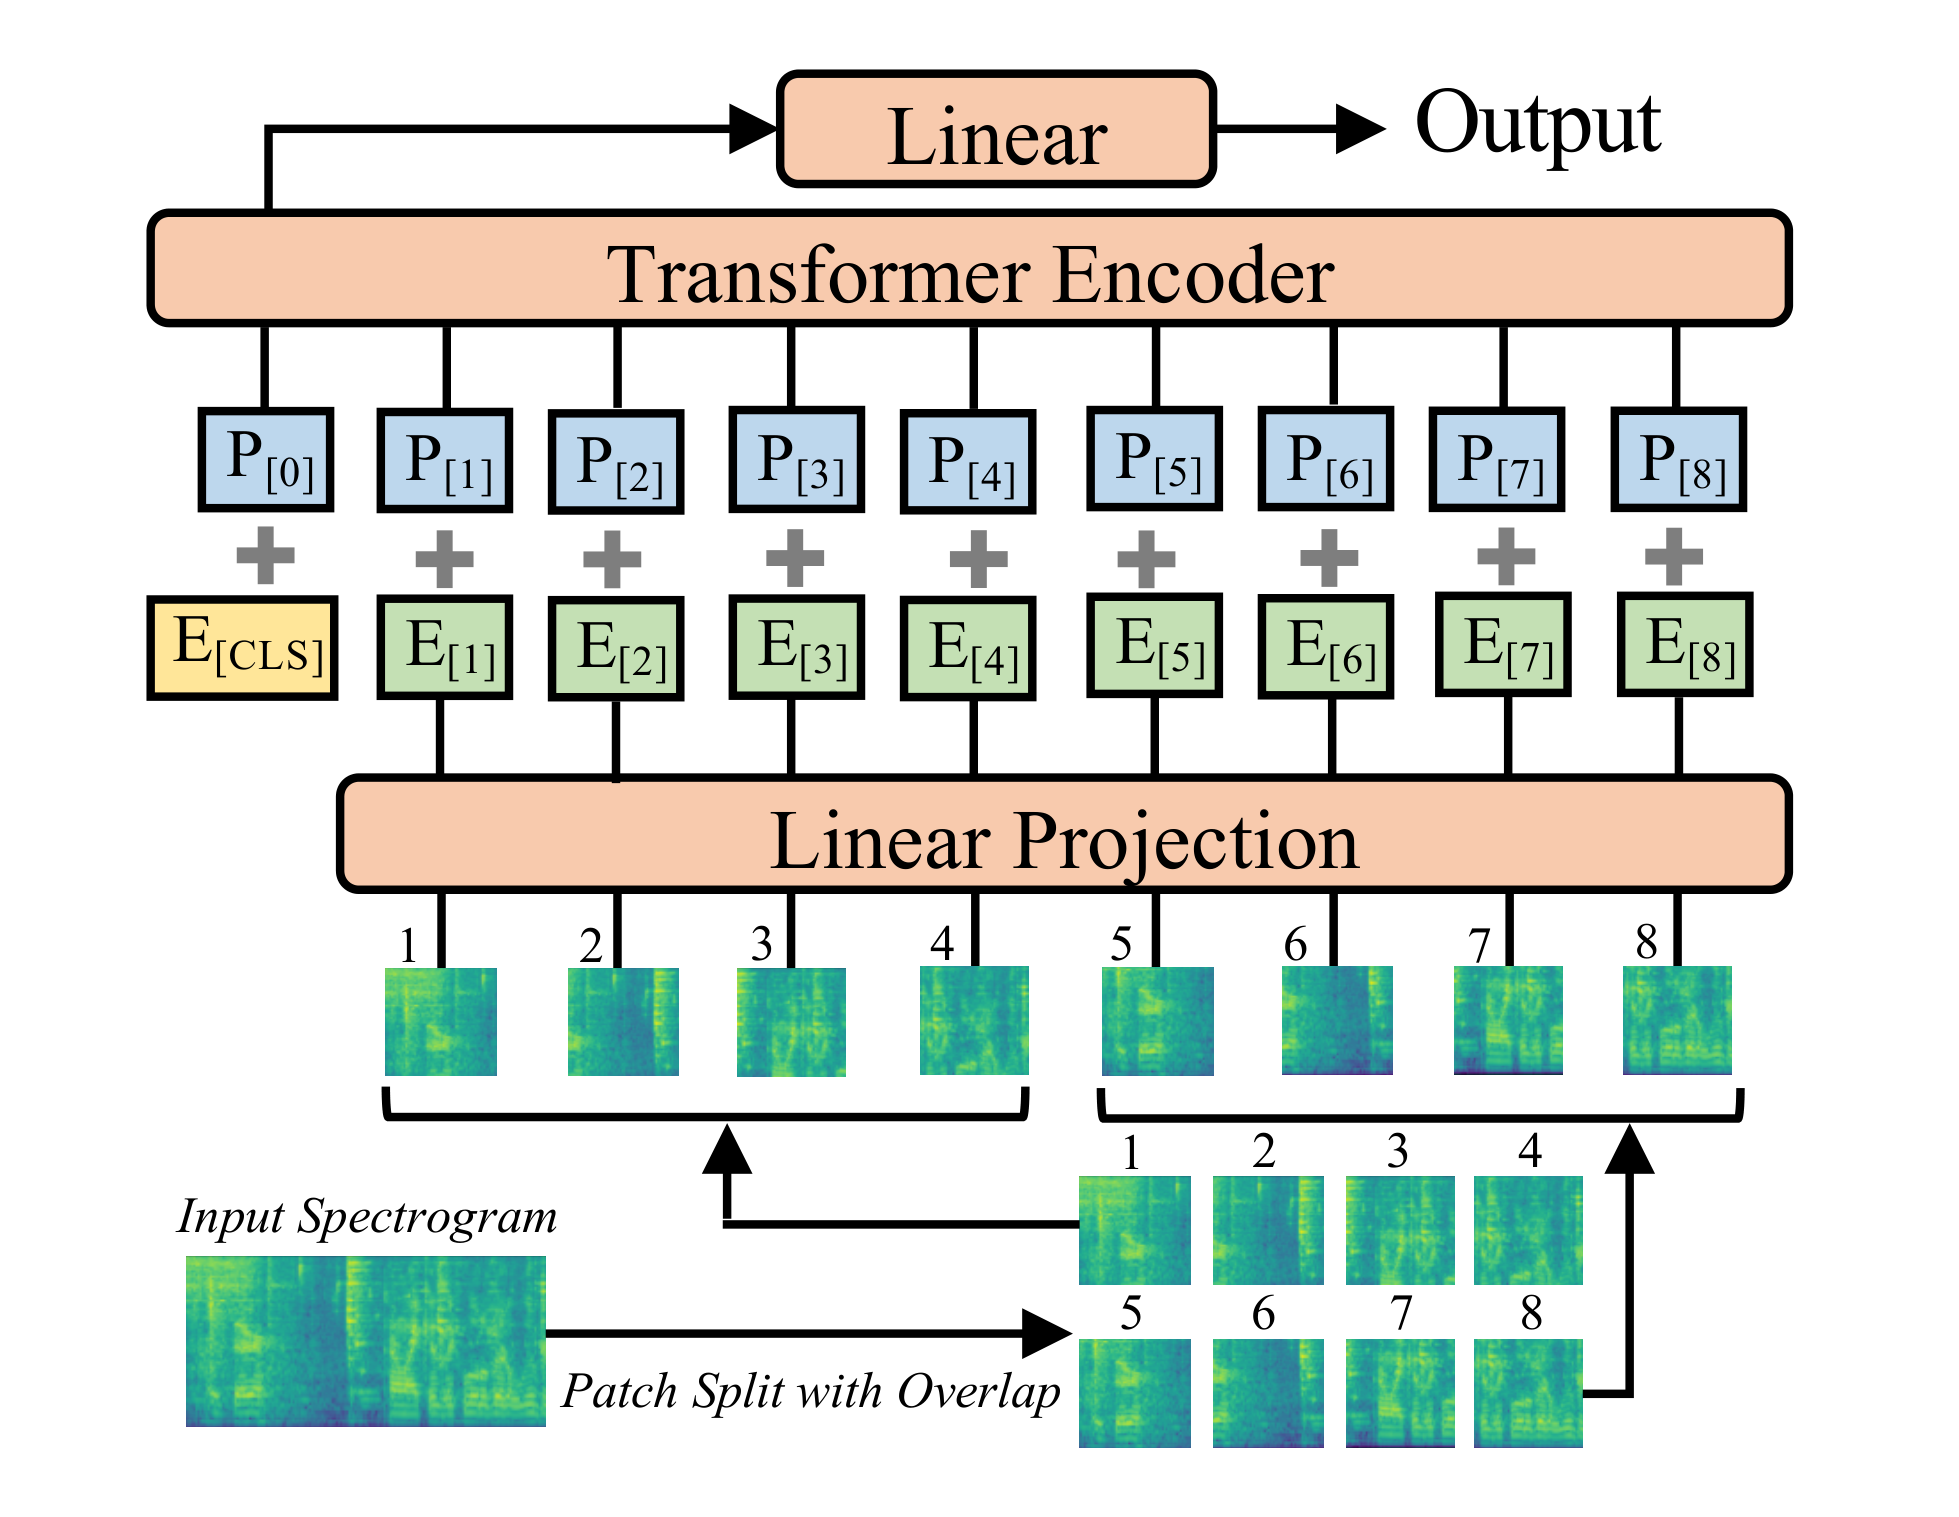
\includegraphics[width=0.62\textwidth]{fig_ast_gong2021.png}
  \caption{Arquitectura del \textit{Audio Spectrogram Transformer}: el
  espectrograma se divide en parches de $16\times16$ con solapamiento, cada
  parche se proyecta linealmente y, con su embedding posicional y el token de
  clase, atraviesa el codificador \textit{Transformer}; la salida del token
  de clase alimenta la capa de clasificación. Tomada de \citet{gong2021ast}.}
  \label{fig:ast}
\end{figure}

%-----------------------------------------------------------------------
\section{\textit{Transfer learning} y \textit{frozen embeddings}}\label{sec:teoria-transfer}

Una red entrenada con millones de imágenes naturales aprende en sus primeras
capas rasgos genéricos (bordes, texturas) y en las últimas rasgos propios de
su tarea. Para un problema nuevo con pocos datos, el \textit{transfer
learning} reutiliza esa red preentrenada: se reemplaza la capa de
clasificación por una de $K$ salidas y se reentrena toda la red con una tasa
de aprendizaje pequeña (\textit{fine-tuning}), o bien se congela el cuerpo
de la red y se entrena solo la nueva capa
\citep[pp.~189--190]{bishop2024deep}. El segundo caso equivale a usar la red
como extractor de características fijas, sus \textit{frozen embeddings}, y
ajustar un clasificador lineal encima. Es la referencia de bajo costo que
\citet{ghani2023embeddings} proponen para bioacústica y uno de los
\textit{baselines} de esta tesis. Aquí se ajustan por completo una
EfficientNet-B0 de ImageNet para audio, una EfficientNet-B3 de ImageNet para
imagen y un AST preentrenado en AudioSet, y ese ajuste se compara con los
\textit{frozen embeddings} de los mismos modelos; como comparación en imagen
se ajusta además un ViT-S/16 preentrenado en ImageNet-21k.

%-----------------------------------------------------------------------
\section{Del audio al espectrograma log-mel}\label{sec:teoria-audio}

\subsection{Señal, muestreo y transformada de Fourier}

Un sonido es una variación de la presión del aire en el tiempo. Al grabarlo,
el computador lo muestrea: lee el valor de la señal $F_s$ veces por segundo
(la \emph{frecuencia de muestreo}; la CNN de esta tesis trabaja a
\SI{32}{\kilo\hertz}), lo
que da una secuencia de números $x(n)$. El teorema de muestreo garantiza que
no se pierde información si la señal no contiene frecuencias superiores a
$F_s/2$, la frecuencia de Nyquist \citep[pp.~50, 61]{muller2021fmp}. Con
\SI{32}{\kilo\hertz} se cubren hasta \SI{16}{\kilo\hertz}, suficiente para
las vocalizaciones de aves, que rara vez superan los
\SIrange{10}{12}{\kilo\hertz}.

La forma de onda muestra cuándo suena algo pero oculta qué frecuencias
contiene. La transformada de Fourier hace lo contrario
\citep[pp.~39--41]{muller2021fmp}. Compara la señal con sinusoides de cada
frecuencia: el coeficiente es grande cuando la señal ``sube y baja'' al
ritmo de esa sinusoide. Para una secuencia de $L$ muestras, la transformada
discreta de Fourier (DFT) es \citep[p.~52]{muller2021fmp}
\begin{equation}
  X(k) = \sum_{n=0}^{L-1} x(n)\, e^{-2\pi i k n / L}, \qquad k = 0, \dots, L-1,
  \label{eq:dft}
\end{equation}
donde el índice $k$ corresponde a la frecuencia física $k F_s / L$ hercios.
Para no perder el ``cuándo'', la transformada de Fourier de tiempo corto
(STFT) aplica la DFT a tramos cortos de la señal: se multiplica la señal por
una ventana $w$ de $L$ muestras (en la CNN, $L = 1024$, \SI{32}{\milli\second}),
se calcula la DFT y se desplaza la ventana en pasos de $H$ muestras ($H
= 320$, \SI{10}{\milli\second}) \citep[pp.~53--55]{muller2021fmp}:
\begin{equation}
  \mathcal{X}(m, k) = \sum_{n=0}^{L-1} x(n + mH)\, w(n)\, e^{-2\pi i k n / L}.
  \label{eq:stft}
\end{equation}
El \emph{espectrograma} es la potencia $|\mathcal{X}(m,k)|^2$ dibujada como
imagen, con el tiempo en horizontal (cuadro $m$, cada \SI{10}{\milli\second})
y la frecuencia en vertical. La ventana impone
un compromiso: cuanto más larga, mejor resuelve las frecuencias y peor los
instantes, y viceversa. Ninguna ventana localiza ambas cosas con precisión
arbitraria \citep[pp.~100--102]{muller2021fmp}. Los \SI{32}{\milli\second}
elegidos resuelven los trinos rápidos de las aves con una resolución en
frecuencia de \SI{31}{\hertz}.

\subsection{Escala mel, logaritmo y normalización}

El espectrograma lineal es ``demasiado genérico'': el oído no resuelve igual
todas las frecuencias ni percibe la intensidad de forma lineal
\citep[pp.~21, 76]{virtanen2018casse}. La percepción del tono es
aproximadamente logarítmica: 220, 440 y \SI{880}{\hertz} suenan ``igual de
distantes'' entre sí \citep[p.~22]{muller2021fmp}. La escala mel formaliza
esa percepción con una fórmula empírica \citep{oshaughnessy1987speech}:
\begin{equation}
  \mathrm{mel}(f) = 2595 \log_{10}\!\left(1 + \frac{f}{700}\right).
  \label{eq:mel}
\end{equation}
Sobre esa escala se define un banco de $M = 128$ filtros triangulares
$\mathbf{B} \in \mathbb{R}^{M \times (L/2+1)}$, estrechos en los graves y anchos
en los agudos (\figref{fig:representacion-audio}c), que agrupan los
coeficientes de la STFT en bandas. La energía de cada banda se comprime con
un logaritmo, porque el rango dinámico del espectrograma es enorme y la
escala logarítmica hace visibles los componentes débiles pero relevantes
\citep[pp.~56, 99]{muller2021fmp}:
\begin{equation}
  X_{\mathrm{mel}}(m, j) = 10 \log_{10}\!\Big(\sum_{k} B_{jk}\, |\mathcal{X}(m, k)|^2 + \delta\Big),
  \qquad j = 1, \dots, M,
  \label{eq:logmel}
\end{equation}
con $\delta$ una constante pequeña que evita el logaritmo de cero. El
resultado, el espectrograma log-mel, es compacto y basta por sí solo como
entrada a una red \citep[p.~81]{virtanen2018casse}. Antes de entrar a la
red se estandariza (media cero y varianza uno), lo que mantiene la primera
capa en zona no saturada. Una ventana de
\SI{5}{\second} (\num{160000} muestras) produce así, con relleno simétrico
de $L/2$ muestras en los bordes, $\lfloor 160000/320 \rfloor + 1 = 501$
cuadros: una ``imagen'' de $128 \times 501$ valores.
Tratarla con una CNN tiene sentido porque, con el eje de frecuencia
logarítmico, un filtro de pocas bandas cubre siempre la misma razón de
frecuencias y puede aprender patrones espectrotemporales invariantes a
pequeñas transposiciones \citep[p.~132]{virtanen2018casse}. El AST usa
su propio \textit{front-end}, el mismo con que fue preentrenado en AudioSet:
remuestrea cada ventana de \SI{10}{\second} a \SI{16}{\kilo\hertz} y
calcula un log-mel de 128 bandas con ventana de \SI{25}{\milli\second} y
paso de \SI{10}{\milli\second} (1\,024 cuadros). La
\figref{fig:representacion-audio} ilustra toda la cadena con una grabación
real del corpus y la \figref{fig:pipeline-audio} la resume.

\begin{figure}[!htb]
  \centering
  \IfFileExists{figuras/fig_representacion_audio.pdf}{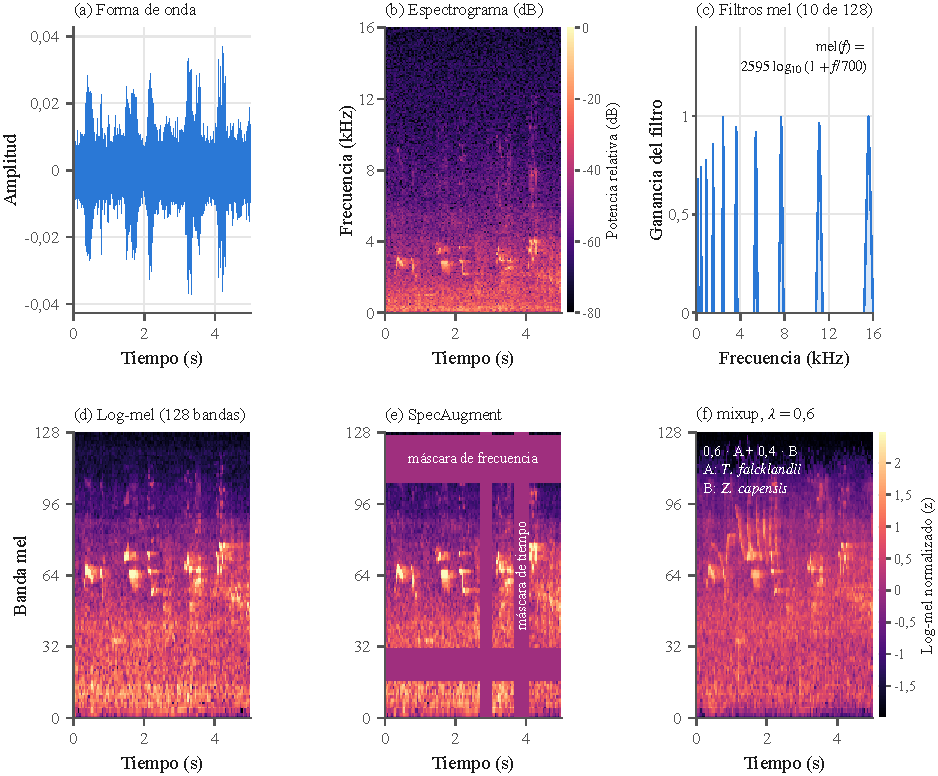
\includegraphics[width=\textwidth]{fig_representacion_audio}}{\fbox{figura pendiente}}
  \caption{Representación de entrada del clasificador de cantos para
  una ventana de \SI{5}{\second} de zorzal (\textit{Turdus falcklandii},
  XC954086): (a) forma de onda; (b) espectrograma de potencia; (c) diez de
  los 128 filtros del banco mel; (d) espectrograma log-mel de $128\times501$
  que recibe la CNN; (e) SpecAugment y (f) \textit{mixup} con una ventana
  de chincol, las dos aumentaciones de entrenamiento.}
  \label{fig:representacion-audio}
\end{figure}

\begin{figure}[H]
  \centering
  \resizebox{\textwidth}{!}{%
  \begin{tikzpicture}[
    node distance=6mm,
    paso/.style={draw, rounded corners, align=center, minimum height=9mm,
                 minimum width=23mm, font=\small, fill=black!5},
    aug/.style={paso, fill=miaamarillo!30},
    mod/.style={paso, fill=pucazul!15},
    flecha/.style={-{Latex[length=2mm]}, thick}]
    \node[paso] (a) {Audio\\Xeno-canto};
    \node[paso, right=of a] (b) {Mono,\\\SI{32}{kHz}};
    \node[paso, right=of b] (c) {Ventanas\\de \SI{5}{s}};
    \node[paso, right=of c] (d) {STFT +\\banco mel};
    \node[paso, right=of d] (e) {$\log(\cdot)$,\\estandarizar};
    \node[aug, below=of e] (f) {SpecAugment,\\mixup, ruido};
    \node[mod, right=of e] (g) {CNN};
    \node[paso, right=of g] (h) {Promedio\\ventanas};
    \draw[flecha] (a)--(b); \draw[flecha] (b)--(c); \draw[flecha] (c)--(d);
    \draw[flecha] (d)--(e); \draw[flecha] (e)--(g); \draw[flecha] (g)--(h);
    \draw[flecha, dashed] (e)--(f); \draw[flecha, dashed] (f)-|(g);
    \node[below=1mm of f, font=\scriptsize] {(solo en entrenamiento)};
  \end{tikzpicture}}
  \caption{Pipeline de procesamiento de audio de la CNN, desde la grabación
  original hasta la predicción a nivel de grabación. El AST sigue el mismo
  esquema con ventanas de \SI{10}{\second} remuestreadas a
  \SI{16}{\kilo\hertz} y su propio banco de filtros.}
  \label{fig:pipeline-audio}
\end{figure}

%-----------------------------------------------------------------------
\section{Protocolos de inferencia: ventanas, agregación y TTA}\label{sec:teoria-inferencia}

Las redes convolucionales con capa densa necesitan una entrada de tamaño
fijo, pero las grabaciones duran desde un segundo hasta varios minutos. Por
eso el modelo clasifica \emph{ventanas} de duración fija (\SI{5}{\second} en
la CNN, \SI{10}{\second} en el AST), y la predicción de una grabación se
obtiene recolectando y agregando las predicciones de sus ventanas, cuidando
que la evaluación se haga a nivel de grabación y no de ventana. Si una
grabación produce $W$ ventanas
$x^{(1)}, \dots, x^{(W)}$, la regla de agregación usada es el promedio de
probabilidades seguido del máximo \citep[pp.~26, 30]{virtanen2018casse}:
\begin{equation}
  \bar{p}_k = \frac{1}{W} \sum_{w=1}^{W} p(\mathcal{C}_k \mid x^{(w)}),
  \qquad \hat{y} = \argmax_k \bar{p}_k.
  \label{eq:agregacion}
\end{equation}
El promedio diluye las ventanas sin vocalización o con ruido entre las que sí
contienen al ave, lo que lo hace robusto a la anotación débil de Xeno-canto,
donde la especie está etiquetada para la grabación completa pero no para
cada instante (\secref{sec:rel-audio}). En esta tesis se reportan dos
protocolos: \emph{ventana única}, que clasifica solo la ventana central
($W = 1$), y \emph{agregado}, con hasta $W = 12$ ventanas de \SI{5}{\second}
equiespaciadas que cubren la grabación en la CNN, y hasta $W = 8$ de
\SI{10}{\second} en el AST (\figref{fig:ventanas-tta}a).

Para la imagen el análogo es la \emph{aumentación en tiempo de prueba}
(TTA): en lugar de clasificar un solo recorte central de la fotografía, se
clasifican diez vistas (los recortes de las cuatro esquinas y del centro, y
sus reflejos horizontales) y se promedian las probabilidades con la misma
Ecuación~\ref{eq:agregacion} (\figref{fig:ventanas-tta}b). Es la aumentación
de datos aplicada en inferencia: suaviza errores debidos al encuadre a cambio
de diez pasadas por el modelo.

\begin{figure}[!htb]
  \centering
  \IfFileExists{figuras/tikz_ventanas_tta.tex}{\fitwidth{\begin{tikzpicture}[x=1mm, y=1mm, font=\footnotesize,
    bloque/.style={draw, rounded corners, align=center, minimum height=9mm,
                   minimum width=24mm, font=\footnotesize, inner xsep=1mm},
    modelo/.style={bloque, fill=miaamarillo!30},
    proc/.style={bloque, fill=black!5, minimum width=26mm},
    salida/.style={bloque, fill=green!12, minimum width=16mm},
    flecha/.style={-{Latex[length=2mm]}, thick},
    etiq/.style={font=\scriptsize, align=center, inner sep=0.3mm},
    % pila de K vectores de probabilidad (icono)
    pics/probvec/.style={code={
      \foreach \d in {2.0,1.0} {\draw[fill=white, thin] (\d,\d) rectangle ++(9,6);}
      \draw[fill=white, thin] (0,0) rectangle (9,6);
      \foreach \bx/\bh in {0.9/1.2, 2.2/0.7, 3.5/4.6, 4.8/1.0, 6.1/1.9, 7.4/0.8}
        {\fill[pucazul!80] (\bx,0.5) rectangle ++(1.0,\bh);}
    }}]

  % ================= (a) AUDIO =================
  \node[anchor=west, inner sep=0] at (0,7.5)
    {\textbf{(a)} Audio: grabación de \SI{45}{s} a \SI{32}{kHz}};
  % barra de la grabación (45 mm = 45 s) con forma de onda estilizada
  \begin{scope}
    \draw[fill=pucazul!15, thin, rounded corners=0.8mm] (0,-3.5) rectangle (45,3.5);
    \clip (0,-3.5) rectangle (45,3.5);
    \draw[pucazul!60!black, line width=0.3pt]
      plot[domain=0:45, samples=320, smooth]
      (\x, {(0.22 + 2.7/(1+((\x-10)/2.2)^2) + 2.2/(1+((\x-24)/1.8)^2)
            + 2.0/(1+((\x-37)/1.6)^2)) * (0.7+0.3*sin(\x*73)) * sin(\x*300)});
  \end{scope}
  % K = 9 ventanas contiguas de 5 s (5 mm cada una)
  \foreach \i in {0,...,8} {
    \draw[fill=black!5, thin] ({\i*5},-8) rectangle ({\i*5+5},-4.5);
  }
  \draw[fill=miaamarillo!30, thick] (20,-8) rectangle (25,-4.5);
  \node[etiq, anchor=north west, align=left] at (0,-9.3)
    {$W=9$ ventanas de \SI{5}{s}, equiespaciadas ($W\le 12$)\\
     amarillo: \emph{ventana única} (central)};

  % pipeline (a), centrado en y=-2
  % llave: cada una de las K ventanas (no la grabación entera) entra a la CNN
  \draw[decorate, decoration={brace, amplitude=1.2mm}, thin] (46,3.5) -- (46,-8);
  \node[modelo] (cnn) at (72.5,-2) {CNN de audio\\EfficientNet-B0\\+ softmax};
  \draw[flecha] (48.2,-2.25) -- (cnn.west |- 0,-2.25)
    node[midway, above=0.4mm, etiq] {log-mel}
    node[midway, below=0.4mm, etiq] {$128{\times}501$};
  \pic at (88,-6.5) {probvec};
  \node[etiq, anchor=north] at (93.5,-7.6) {$W$ vectores\\$p^{(w)}\in\mathbb{R}^{55}$};
  \draw[flecha] (cnn.east) -- (87.6,-2);
  \node[proc] (prom) at (117.5,-2) {Promedio\\$\bar{p}=\frac{1}{W}\sum_{w} p^{(w)}$};
  \draw[flecha] (100.4,-2) -- (prom.west);
  \node[salida] (esp) at (149,-2) {Especie\\$\hat{y}$};
  \draw[flecha] (prom.east) -- (esp.west) node[midway, above=0.4mm, etiq] {$\arg\max$};

  % ================= (b) IMAGEN =================
  \node[anchor=west, inner sep=0] at (0,-23)
    {\textbf{(b)} Imagen: fotografía redimensionada (lado menor a \SI{441}{px})};
  % fotografía real del corpus (chucao, iNaturalist, CC BY-NC 4.0), recortada a 28 x 21 mm
  \begin{scope}
    \clip (8,-46.5) rectangle (36,-25.5);
    \node[inner sep=0] at (22,-36) {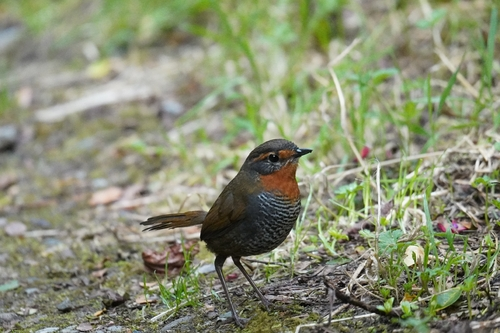
\includegraphics[height=21mm]{fig_tta_foto.jpg}};
  \end{scope}
  \draw[thin, black!40] (8,-46.5) rectangle (36,-25.5);
  % 4 recortes de esquina (azul, discontinuo): cuadrados de 15 x 15 mm, solapados
  \foreach \px/\py in {8/-25.5, 21/-25.5, 8/-31.5, 21/-31.5} {
    \draw[pucazul!70!black, dash pattern=on 1.2pt off 0.9pt, line width=0.5pt]
      (\px,\py) rectangle ++(15,-15);
  }
  % recorte central (amarillo, continuo), cuadrado de 15 x 15 mm
  \draw[miaamarillo!80!black, thick] (14.5,-28.5) rectangle ++(15,-15);
  \node[etiq, anchor=north west, align=left] at (0,-47.8)
    {5 recortes de $384{\times}384$ px: 4 esquinas + centro\\
     amarillo: \emph{recorte central} (1 vista)};

  % pipeline (b), centrado en y=-36
  \node[modelo] (b3) at (72.5,-36) {CNN de imagen\\EfficientNet-B3\\+ softmax};
  \draw[flecha] (36.4,-36) -- (b3.west)
    node[midway, above=0.4mm, etiq] {$\times 2$ volteo\\horizontal}
    node[midway, below=0.4mm, etiq] {$= 10$ vistas};
  \pic at (88,-40.5) {probvec};
  \node[etiq, anchor=north] at (93.5,-41.6) {10 vectores\\$p^{(v)}\in\mathbb{R}^{53}$};
  \draw[flecha] (b3.east) -- (87.6,-36);
  \node[proc] (promb) at (117.5,-36) {Promedio (TTA)\\$\bar{p}=\frac{1}{10}\sum_{v} p^{(v)}$};
  \draw[flecha] (100.4,-36) -- (promb.west);
  \node[salida] (espb) at (149,-36) {Especie\\$\hat{y}$};
  \draw[flecha] (promb.east) -- (espb.west) node[midway, above=0.4mm, etiq] {$\arg\max$};
\end{tikzpicture}
}}{\fbox{figura pendiente}}
  \caption{Protocolos de inferencia. (a) Audio: la grabación se divide en
  ventanas de \SI{5}{\second}, cada una pasa por la CNN y las probabilidades
  se promedian (Ecuación~\ref{eq:agregacion}); la \emph{ventana única} usa
  solo la central (en amarillo). (b) Imagen: cinco recortes de $384\times384$
  y sus volteos horizontales forman las diez vistas de la TTA; el
  \emph{recorte central} usa una sola (en amarillo). Fotografía de chucao de
  pmarinaraya (iNaturalist, CC BY-NC 4.0).}
  \label{fig:ventanas-tta}
\end{figure}

%-----------------------------------------------------------------------
\section{Fusión multimodal}\label{sec:teoria-fusion}

Sea $\mathcal{Y} = \{1, \dots, K\}$ el conjunto de especies. Cada observación
consiste en una señal de audio $x^{(a)}$ y/o una imagen $x^{(v)}$, con
etiqueta $y \in \mathcal{Y}$. Se entrenan dos clasificadores independientes,
$f_a$ y $f_v$, cada uno con su propia red y su propio conjunto de datos, que
producen las probabilidades $p_a(k \mid x^{(a)})$ y $p_v(k \mid x^{(v)})$ con
la Ecuación~\ref{eq:softmax}. Las tres formas de combinar las modalidades
\citep{baltrusaitis2019multimodal} se distinguen por el nivel en que ocurre
la combinación (\figref{fig:fusion-estrategias}).

\begin{itemize}[leftmargin=*, itemsep=2pt]
  \item \textbf{\textit{Early fusion}.} Se concatenan las representaciones
        internas de ambas ramas (sus \textit{embeddings} $\mathbf{h}_a \in
        \mathbb{R}^{1280}$ y $\mathbf{h}_v \in \mathbb{R}^{1536}$) y un único
        clasificador $g$ decide: $\hat{y} = \argmax_k g([\mathbf{h}_a;
        \mathbf{h}_v])_k$. Puede modelar interacciones entre modalidades,
        pero exige que ambas estén presentes.
  \item \textbf{\textit{Intermediate fusion}.} Cada \textit{embedding} pasa
        primero por una proyección propia a un espacio común de 256
        dimensiones y la concatenación de las proyecciones alimenta el
        clasificador. Agrega parámetros que deben aprenderse de los datos
        emparejados.
  \item \textbf{\textit{Late fusion}.} Cada rama decide por su cuenta y se
        combinan las probabilidades con una media ponderada por $\alpha \in
        [0, 1]$:
        \begin{equation}
          \hat{y} = \argmax_{k \in \mathcal{Y}} \;
          \alpha\, p_a(k \mid x^{(a)}) + (1-\alpha)\, p_v(k \mid x^{(v)}).
          \label{eq:fusion}
        \end{equation}
        Si falta una modalidad, $\hat{y}$ se obtiene de la otra, lo que hace
        al sistema robusto a modalidades faltantes y permite entrenar cada
        rama con datos no emparejados. Una alternativa es la media
        geométrica, $\propto p_a^{\alpha}\, p_v^{1-\alpha}$ (un producto de
        expertos). Con $\alpha = 1/2$ y un prior uniforme sobre las especies
        equivale, salvo normalización, a la combinación \textit{naive Bayes}
        $p(\mathcal{C}_k \mid x^{(a)})\, p(\mathcal{C}_k \mid x^{(v)}) /
        p(\mathcal{C}_k)$, que supone las dos modalidades condicionalmente
        independientes dada la especie \citep[pp.~146--147]{bishop2024deep}.
        Penaliza más a las clases que una modalidad descarta con seguridad.
\end{itemize}

\begin{figure}[!htb]
  \centering
  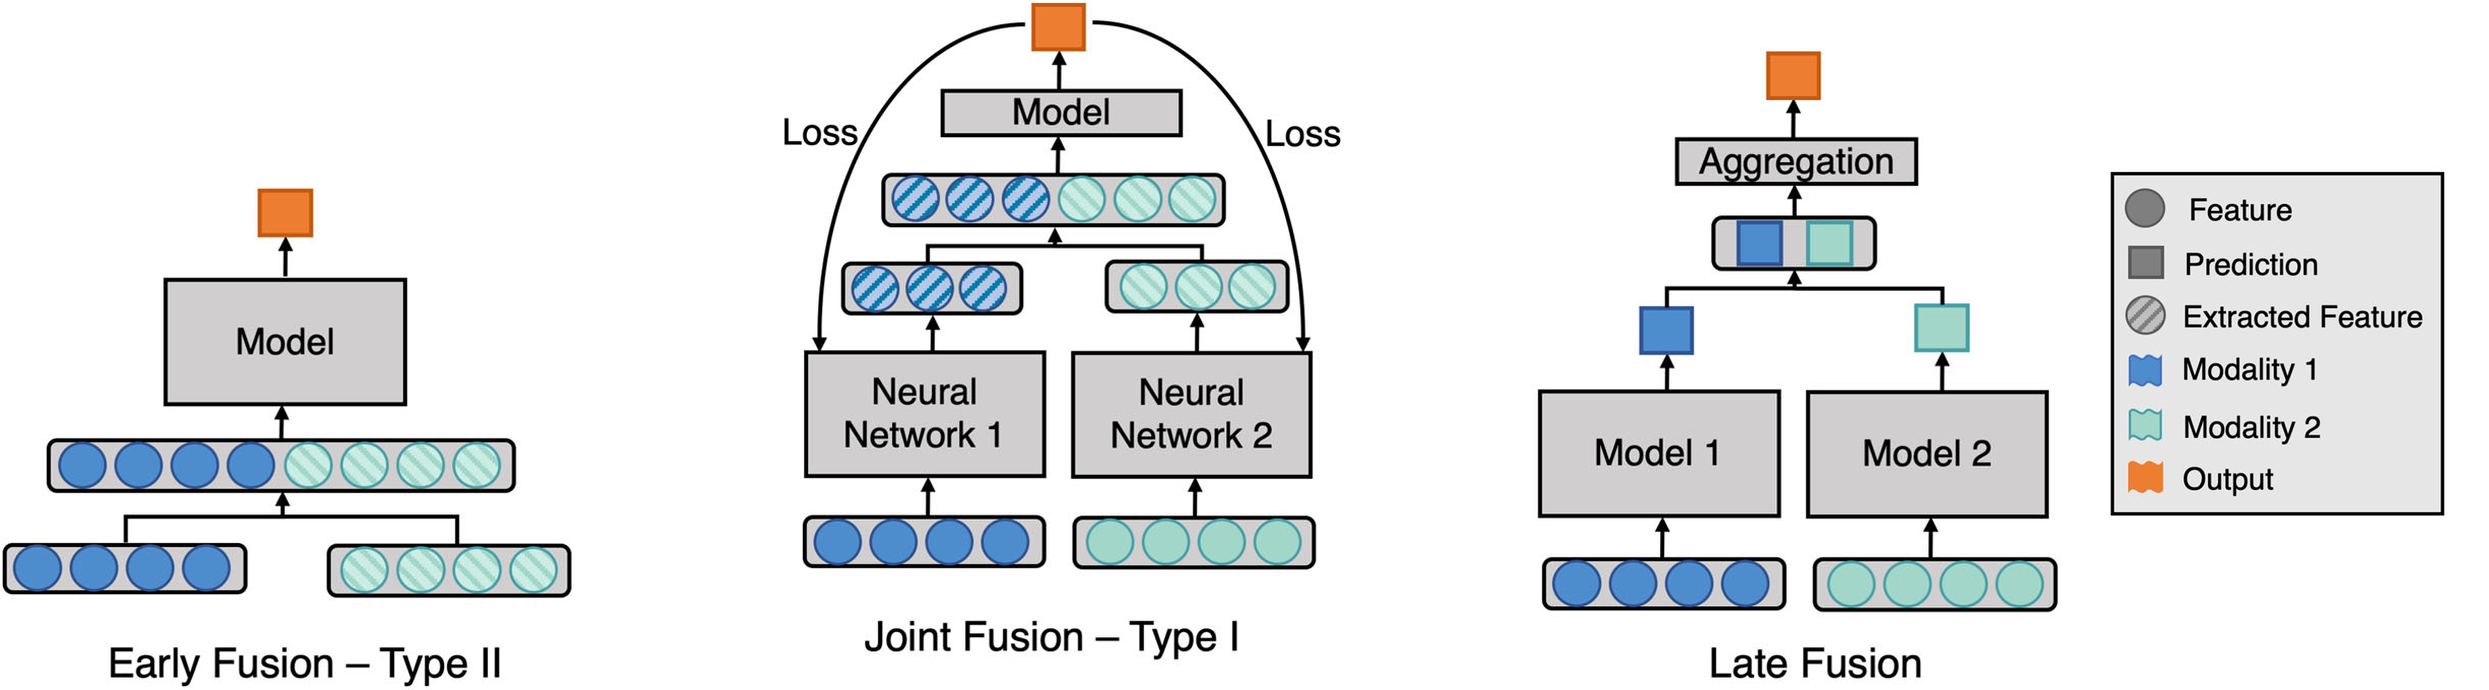
\includegraphics[width=\textwidth]{fig_fusion_huang2020.png}
  \caption{Estrategias de fusión multimodal: \textit{early fusion}
  (se concatenan las características extraídas de cada modalidad),
  \textit{joint fusion}, que corresponde a la \textit{intermediate fusion}
  de esta tesis (cada modalidad pasa por su propia red antes de
  concatenarse), y \textit{late fusion} (cada modalidad predice por separado
  y las predicciones se agregan). Los subtipos I y II distinguen si las
  características de entrada son crudas o extraídas. Tomada de
  \citet{huang2020fusion}, CC BY 4.0.}
  \label{fig:fusion-estrategias}
\end{figure}

\textbf{Evaluación con fuentes no emparejadas.} Las grabaciones de
Xeno-canto y las fotografías de iNaturalist no corresponden a los mismos
individuos, de modo que no existen pares naturales de audio e imagen. Para
evaluar la fusión se construyen pares sintéticos: cada grabación del
conjunto de prueba de audio se empareja al azar con una fotografía del
conjunto de prueba de imagen de la misma especie, repitiendo el
emparejamiento varias veces y reportando media y desviación estándar de las
métricas. Este protocolo mide la ganancia de combinar evidencia de ambas
modalidades, que es el escenario de uso previsto (un observador que dispone
de una grabación y una fotografía de la misma ave), pero no captura
correlaciones entre el canto y la apariencia de un mismo individuo. Esta
limitación se declara en el análisis de resultados.

%-----------------------------------------------------------------------
\section{Modelos de distribución de especies}\label{sec:teoria-sdm}

\subsection{Qué modela un modelo de distribución}

Un modelo de distribución de especies (SDM, o modelo de idoneidad de
hábitat) relaciona empíricamente las observaciones de una especie con las
condiciones ambientales de los sitios donde se la observó, y proyecta esa
relación a todo el territorio para estimar dónde podría estar
\citep[p.~11]{guisan2017hsdm}. Lo que captura es el \emph{nicho realizado}:
el conjunto de condiciones (temperatura, precipitación, vegetación,
altitud) en que la especie efectivamente se encuentra, una vez descontadas
la competencia y la historia, que es lo único observable con datos de campo
\citep[pp.~32, 36]{guisan2017hsdm}. El modelo supone que la especie está en
pseudoequilibrio con su ambiente y que la muestra cubre los ambientes que
ocupa. Por ser correlativo, apoya hipótesis pero no las prueba
\citep[pp.~46, 53]{guisan2017hsdm}. Formalmente, para cada especie $k$ se
dispone de presencias $\mathcal{P}_k = \{(s_i, t_i)\}$, con $s_i$ la
ubicación y $t_i$ la fecha, y cada punto se describe con un vector de
covariables $\mathbf{c}(s, t) \in \mathbb{R}^d$: temperatura media anual y
precipitación anual de WorldClim, elevación, NDVI y la codificación cíclica
del mes, $(\sin 2\pi t/12, \cos 2\pi t/12)$, que deja diciembre y enero
contiguos. El NDVI (índice de vegetación de diferencia normalizada) mide el
``verdor'' a partir de la luz que refleja la superficie en dos bandas del
espectro \citep{tucker1979ndvi}:
\begin{equation}
  \mathrm{NDVI} = \frac{\rho_{\mathrm{NIR}} - \rho_{\mathrm{Red}}}{\rho_{\mathrm{NIR}} + \rho_{\mathrm{Red}}},
  \label{eq:ndvi}
\end{equation}
donde $\rho_{\mathrm{NIR}}$ y $\rho_{\mathrm{Red}}$ son las \emph{reflectancias}
(fracción de la luz incidente que la superficie devuelve) en el infrarrojo
cercano y en el rojo. La vegetación verde refleja mucho infrarrojo y absorbe
el rojo, así que su NDVI se acerca a uno, mientras que el suelo desnudo, el
agua y la nieve dan valores cercanos a cero o negativos. Índices como este
``realzan'' una señal que las bandas por separado ocultan
\citep[p.~98]{guisan2017hsdm}.

\subsection{Datos de solo presencia y pseudoausencias}

Los registros de ciencia ciudadana son de \emph{solo presencia}: dicen dónde
se vio a la especie, nunca dónde se la buscó sin éxito. Un modelo que
contraste presencias con ausencias necesita entonces puntos de contraste
artificiales, los \emph{puntos de fondo} o \emph{pseudoausencias}, que
representan las condiciones ambientales disponibles en el territorio
\citep[pp.~131--134]{guisan2017hsdm}. La opción con menos supuestos es
muestrearlos al azar por toda el área de estudio. Pero los datos
oportunistas no se recogen al azar: se agrupan en zonas accesibles y a lo
largo de las vías de comunicación \citep[p.~56]{guisan2017hsdm}, y ese
sesgo de GBIF ha crecido con el tiempo. Con
un fondo uniforme el modelo aprende dónde hay observadores, no dónde hay
hábitat. El método del \emph{grupo objetivo} corrige el sesgo tomando como
pseudoausencias los registros de otras especies del mismo grupo (aquí, las
demás aves del conjunto), porque esos registros comparten exactamente el
esfuerzo de observación de las presencias \citep{phillips2009bias}. La
\figref{fig:fondo-objetivo} muestra la diferencia con los datos de esta
tesis.

\begin{figure}[!htb]
  \centering
  \IfFileExists{figuras/fig_fondo_objetivo.pdf}{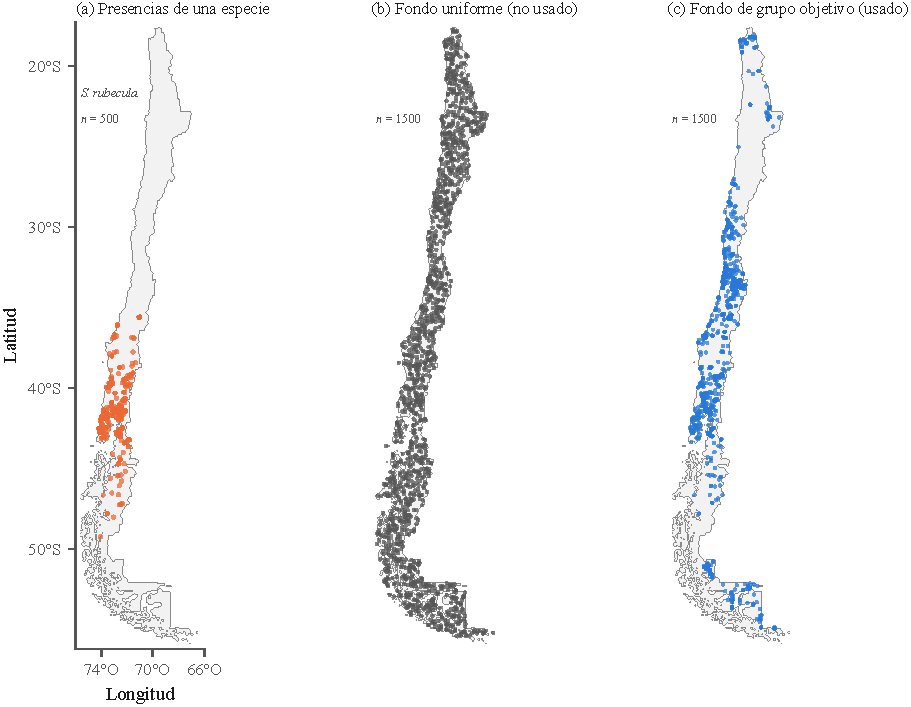
\includegraphics[width=\textwidth]{fig_fondo_objetivo}}{\fbox{figura pendiente}}
  \caption{Presencias y pseudoausencias del modelo de distribución:
  (a) 500 registros de chucao (\textit{Scelorchilus rubecula}); (b) fondo
  uniforme sobre Chile continental, descartado; (c) fondo de grupo objetivo,
  tomado de los avistamientos de las demás aves del conjunto, que reproduce
  la geografía del esfuerzo de observación y es el que usa la tesis.}
  \label{fig:fondo-objetivo}
\end{figure}

\subsection{MaxEnt y la regresión logística}

MaxEnt es el método de referencia para datos de solo presencia. Su idea: de
todas las distribuciones de probabilidad sobre el territorio compatibles con
lo observado, elegir la de máxima entropía, la más ``neutra''
\citep[p.~217]{guisan2017hsdm}. En la formulación de
\citet{elith2011maxent}, si $f(\mathbf{c})$ es la densidad de las condiciones
ambientales en el territorio (estimada con los puntos de fondo) y
$f_1(\mathbf{c})$ la densidad en los sitios de presencia, MaxEnt estima el
cociente $f_1(\mathbf{c})/f(\mathbf{c})$ buscando la $f_1$ más cercana a $f$ en
entropía relativa, sujeta a que los promedios de las covariables bajo $f_1$
coincidan con los observados en las presencias. La solución tiene forma
exponencial en una
combinación lineal de \emph{features} $h(\mathbf{c})$ de las covariables
(lineales, cuadráticas, de umbral, etc.) \citep{phillips2006maxent}:
\begin{equation}
  \frac{f_1(\mathbf{c})}{f(\mathbf{c})} = \exp\!\big(\eta(\mathbf{c})\big),
  \qquad \eta(\mathbf{c}) = \beta_0 + \boldsymbol{\beta}^{\mathrm{T}} h(\mathbf{c}),
  \label{eq:maxent}
\end{equation}
ajustada maximizando una verosimilitud penalizada, porque sin
regularización el modelo sobreajusta \citep[p.~219]{guisan2017hsdm}. Esta
forma es la de un modelo lineal generalizado: en el límite de un fondo
grande, contrastar presencias con el fondo mediante una regresión logística
penalizada estima las mismas pendientes $\boldsymbol{\beta}$ (el intercepto
difiere y depende del número de puntos de fondo)
\citep{fithian2013equivalence}. Por eso el \textit{baseline} MaxEnt de esta
tesis se implementa como una regresión logística con \textit{features}
lineales y cuadráticas y penalización L2 (la implementación original de
MaxEnt usa L1):
\begin{equation}
  P(y = 1 \mid \mathbf{c}) = \sigma\!\big(\mathbf{w}^{\mathrm{T}} h(\mathbf{c}) + b\big),
  \qquad \sigma(a) = \frac{1}{1 + e^{-a}},
  \label{eq:logistica}
\end{equation}
donde $\sigma$ es la función logística, que convierte el predictor lineal
(no acotado) en una probabilidad \citep[pp.~165--167]{guisan2017hsdm}. Los
términos cuadráticos producen las respuestas unimodales típicas de las
especies, que rinden mejor cerca de un óptimo ambiental y peor a ambos
lados. La ventaja de este modelo es su
interpretabilidad: cada coeficiente dice cómo cambia la probabilidad de
presencia con una covariable.

\subsection{Árboles de decisión, Random Forest y gradient boosting}

Un \emph{árbol de clasificación} divide los datos repetidamente en dos
grupos según una regla sobre una sola covariable (``NDVI $< 0{,}4$'',
``elevación $> \SI{1200}{\metre}$''), eligiendo en cada nodo la división que
mejor separa presencias de ausencias. Cada hoja guarda la proporción de
presencias que llegan a ella, que es su probabilidad predicha
\citep[p.~190]{guisan2017hsdm}. En la implementación usada, la impureza de
un nodo se mide con el índice de Gini, $G = 1 - p_{\mathrm{pres}}^2 -
p_{\mathrm{aus}}^2$, con $p_{\mathrm{pres}}$ y $p_{\mathrm{aus}}$ las
proporciones de presencias y ausencias en el nodo, y cada división minimiza la impureza ponderada de los dos hijos. El árbol no asume
ninguna forma de respuesta y captura interacciones, pero ajustar un solo
árbol es una operación de alta varianza: pequeños cambios en los datos
producen árboles muy distintos \citep[pp.~194, 203]{guisan2017hsdm}. Los
\emph{ensambles} corrigen eso combinando muchos árboles
(\figref{fig:arboles}).

\begin{figure}[!htb]
  \centering
  \IfFileExists{figuras/tikz_arboles.tex}{\fitwidth{% Ensambles de árboles para el modelo de distribución: (a) Random Forest,
% (b) gradient boosting y (c) MaxEnt como regresión logística penalizada.
% Incluir con \input dentro de un entorno figure (ancho ~157 mm).
% Los tres árboles de (a) son esquemáticos: profundidad 2, reglas y
% probabilidades de hoja ilustrativas (no provienen de un modelo ajustado).
\begin{tikzpicture}[x=1mm, y=1mm, font=\footnotesize,
  caja/.style={draw, rounded corners=1.5pt, align=center, inner sep=2pt, line width=0.4pt},
  datos/.style={caja, fill=pucazul!15},
  proc/.style={caja, fill=black!5},
  modelo/.style={caja, fill=miaamarillo!30},
  salida/.style={caja, fill=green!12},
  regla/.style={modelo, font=\scriptsize, inner xsep=1.2pt, inner ysep=1.5pt, minimum height=4.5mm},
  hoja/.style={salida, circle, font=\scriptsize, inner sep=0.6pt, minimum size=5mm},
  flecha/.style={-{Latex[length=2mm]}, thick},
  flechafina/.style={-{Latex[length=1.5mm]}, semithick},
  rama/.style={semithick, black!60},
  sino/.style={font=\scriptsize, text=black!75, inner sep=0.3pt},
  etq/.style={font=\scriptsize, inner sep=0.8pt},
  titulo/.style={font=\footnotesize\bfseries, anchor=west, inner sep=0},
  pres/.style={circle, fill=pucazul, draw=pucazul!50!black, inner sep=0, minimum size=1.7mm},
  fondo/.style={circle, fill=white, draw=black!60, semithick, inner sep=0, minimum size=1.7mm},
  pics/minitree/.style={code={
      \node[modelo, minimum size=3mm, inner sep=0, rounded corners=1pt] (-r) at (0,0) {};
      \node[salida, circle, minimum size=2.4mm, inner sep=0] (-a) at (-3,-4.5) {};
      \node[salida, circle, minimum size=2.4mm, inner sep=0] (-b) at (3,-4.5) {};
      \draw[rama] (-r) -- (-a); \draw[rama] (-r) -- (-b);}}]

  % ======================= (a) Random Forest =======================
  \node[titulo] at (0,67) {(a) Random Forest: \mdseries bagging de árboles con selección aleatoria de covariables};
  \node[datos] (datos) at (62,60)
    {Conjunto de entrenamiento: presencias ($y{=}1$) y fondo de grupo objetivo ($y{=}0$)\\
     con 6 covariables: NDVI, temperatura, precipitación, elevación, sen/cos del mes};

  % muestras bootstrap
  \node[proc, font=\scriptsize] (b1) at (20,46.5)  {Muestra\\bootstrap 1};
  \node[proc, font=\scriptsize] (b2) at (65,46.5)  {Muestra\\bootstrap 2};
  \node[proc, font=\scriptsize] (b3) at (107,46.5) {Muestra\\bootstrap 3};
  \node[font=\footnotesize] at (128,46.5) {$\cdots$};
  \coordinate (bus) at ($(datos.south)+(0,-1.8)$);
  \draw[thick] (datos.south) -- (bus);
  \draw[thick] (bus -| b1.north) -- (bus -| b3.north);
  \draw[flecha] (bus -| b1.north) -- (b1.north);
  \draw[flecha] (bus -| b2.north) -- (b2.north);
  \draw[flecha] (bus -| b3.north) -- (b3.north);

  % ---- árbol 1 ----
  \node[regla] (r1)  at (20,36.5) {NDVI $<$ 0,4};
  \node[regla] (c11) at (9,28)  {elev. $>$ \SI{1200}{m}};
  \node[regla] (c12) at (31,28) {temp. $>$ \SI{12}{\celsius}};
  \node[hoja] (h11) at (3.5,20.5)  {0,10};
  \node[hoja] (h12) at (14.5,20.5) {0,35};
  \node[hoja] (h13) at (25.5,20.5) {0,80};
  \node[hoja] (h14) at (36.5,20.5) {0,45};
  \draw[rama] (r1) -- (c11) node[sino, pos=0.7, above left=-0.5pt] {sí};
  \draw[rama] (r1) -- (c12) node[sino, pos=0.7, above right=-0.5pt] {no};
  \draw[rama] (c11) -- (h11); \draw[rama] (c11) -- (h12);
  \draw[rama] (c12) -- (h13); \draw[rama] (c12) -- (h14);
  \node[font=\scriptsize] (t1) at (20,15.5) {$T_1(\mathbf{c})$};

  % ---- árbol 2 ---- (los árboles 2 y 3 van 3 mm a la derecha para que las
  % reglas de árboles vecinos no se toquen)
  \begin{scope}[xshift=3mm]
  \node[regla] (r2)  at (62,36.5) {temp. $>$ \SI{12}{\celsius}};
  \node[regla] (c21) at (51,28) {precip. $<$ \SI{300}{mm}};
  \node[regla] (c22) at (73,28) {sen(mes) $>$ 0};
  \node[hoja] (h21) at (45.5,20.5) {0,20};
  \node[hoja] (h22) at (56.5,20.5) {0,65};
  \node[hoja] (h23) at (67.5,20.5) {0,15};
  \node[hoja] (h24) at (78.5,20.5) {0,50};
  \draw[rama] (r2) -- (c21) node[sino, pos=0.7, above left=-0.5pt] {sí};
  \draw[rama] (r2) -- (c22) node[sino, pos=0.7, above right=-0.5pt] {no};
  \draw[rama] (c21) -- (h21); \draw[rama] (c21) -- (h22);
  \draw[rama] (c22) -- (h23); \draw[rama] (c22) -- (h24);
  \node[font=\scriptsize] (t2) at (62,15.5) {$T_2(\mathbf{c})$};
  \end{scope}

  % ---- árbol 3 ----
  \begin{scope}[xshift=3mm]
  \node[regla] (r3)  at (104,36.5) {elev. $>$ \SI{1200}{m}};
  \node[regla] (c31) at (93,28)  {NDVI $<$ 0,4};
  \node[regla] (c32) at (115,28) {precip. $>$ \SI{800}{mm}};
  \node[hoja] (h31) at (87.5,20.5)  {0,05};
  \node[hoja] (h32) at (98.5,20.5)  {0,40};
  \node[hoja] (h33) at (109.5,20.5) {0,70};
  \node[hoja] (h34) at (120.5,20.5) {0,30};
  \draw[rama] (r3) -- (c31) node[sino, pos=0.7, above left=-0.5pt] {sí};
  \draw[rama] (r3) -- (c32) node[sino, pos=0.7, above right=-0.5pt] {no};
  \draw[rama] (c31) -- (h31); \draw[rama] (c31) -- (h32);
  \draw[rama] (c32) -- (h33); \draw[rama] (c32) -- (h34);
  \node[font=\scriptsize] (t3) at (104,15.5) {$T_3(\mathbf{c})$};
  \end{scope}

  \draw[flecha] (b1) -- (r1); \draw[flecha] (b2) -- (r2); \draw[flecha] (b3) -- (r3);


  % promedio
  \node[salida] (prom) at (65,5.5)
    {Promedio de los $B$ árboles: \; $p(\mathbf{c}) = \frac{1}{B}\sum_{b=1}^{B} T_b(\mathbf{c})$};
  \draw[flecha] (t1.south) -- ++(0,-2.5) -| ([xshift=-14mm]prom.north);
  \draw[flecha] (t2.south) -- (prom.north);
  \draw[flecha] (t3.south) -- ++(0,-2.5) -| ([xshift=14mm]prom.north);

  % separadores
  \draw[black!30, dashed] (0,-1) -- (157,-1);
  \draw[black!30, dashed] (107.5,-3) -- (107.5,-56);

  % ======================= (b) Gradient boosting =======================
  \node[titulo] at (0,-5) {(b) Gradient boosting: \mdseries árboles secuenciales sobre el residuo};
  \node[proc] (F0) at (8,-40) {$F_0(\mathbf{c})$\\[-2pt]{\scriptsize constante}};
  \node[proc] (F1) at (30,-40) {$F_1(\mathbf{c})$};
  \node[proc] (F2) at (52,-40) {$F_2(\mathbf{c})$};
  \node[proc] (F3) at (74,-40) {$F_3(\mathbf{c})$};
  \node[inner sep=0.5pt] (Fd) at (86,-40) {$\cdots$};
  \node[salida] (FM) at (97,-40) {$F_J(\mathbf{c})$};
  \node[font=\scriptsize, anchor=north, inner sep=1pt] at ([xshift=-1mm]FM.south) {$p(\mathbf{c})=\sigma\big(F_J(\mathbf{c})\big)$};
  \draw[flecha] (F0) -- (F1); \draw[flecha] (F1) -- (F2); \draw[flecha] (F2) -- (F3);
  \draw[flecha] (F3) -- (Fd); \draw[flecha] (Fd) -- (FM);

  \pic (g1) at (19,-23) {minitree};
  \pic (g2) at (41,-23) {minitree};
  \pic (g3) at (63,-23) {minitree};
  \node[font=\scriptsize] at (19,-17.5) {$T_1(\mathbf{c})$};
  \node[font=\scriptsize] at (41,-17.5) {$T_2(\mathbf{c})$};
  \node[font=\scriptsize] at (63,-17.5) {$T_3(\mathbf{c})$};

  \draw[flechafina, dashed] (F0.north) -- (g1-a.south west)
        node[etq, pos=0.62, left] {$r_1$};
  \draw[flechafina] (g1-b.south east) -- (F1.north)
        node[etq, pos=0.3, right] {$\nu T_1$};
  \draw[flechafina, dashed] (F1.north) -- (g2-a.south west)
        node[etq, pos=0.62, left] {$r_2$};
  \draw[flechafina] (g2-b.south east) -- (F2.north)
        node[etq, pos=0.3, right] {$\nu T_2$};
  \draw[flechafina, dashed] (F2.north) -- (g3-a.south west)
        node[etq, pos=0.62, left] {$r_3$};
  \draw[flechafina] (g3-b.south east) -- (F3.north)
        node[etq, pos=0.3, right] {$\nu T_3$};

  \draw[flechafina, dashed] (2,-48.5) -- (7,-48.5);
  \node[anchor=west, font=\scriptsize] at (7.5,-48.5)
    {pseudorresiduo $r_m = y - \sigma\big(F_{m-1}(\mathbf{c})\big)$ que aprende el árbol $T_m$};
  \draw[flechafina] (2,-52) -- (7,-52);
  \node[anchor=west, font=\scriptsize] at (7.5,-52)
    {$F_m(\mathbf{c}) = F_{m-1}(\mathbf{c}) + \nu\,T_m(\mathbf{c})$, \; $\nu = 0{,}05$, \; $J = 300$};

  % ======================= (c) MaxEnt / regresión logística =======================
  \node[titulo] at (110,-5) {(c) MaxEnt: \mdseries regresión logística};
  % leyenda
  \node[pres] at (118,-10.5) {};
  \node[anchor=west, font=\scriptsize, inner sep=1pt] at (119.5,-10.5) {presencia};
  \node[fondo] at (139,-10.5) {};
  \node[anchor=west, font=\scriptsize, inner sep=1pt] at (140.5,-10.5) {fondo};
  % región de presencia (lado positivo de la frontera)
  \begin{scope}
    \clip (116,-46) rectangle (154,-14);
    \fill[pucazul!8] (116,-22.82) -- (154,-45.18) -- (154,-14) -- (116,-14) -- cycle;
  \end{scope}
  % ejes
  \draw[flechafina, black!70] (116,-46) -- (155,-46);
  \draw[flechafina, black!70] (116,-46) -- (116,-13);
  \node[font=\scriptsize] at (135.5,-48.3) {$h_1(\mathbf{c})$};
  \node[font=\scriptsize, rotate=90] at (113.3,-30) {$h_2(\mathbf{c})$};
  % frontera
  \draw[thick, pucazul!60!black] (116,-22.82) -- (154,-45.18)
    node[pos=0.22, above, sloped, font=\scriptsize, inner sep=0.8pt] {$\mathbf{w}^{\mathrm T} h(\mathbf{c}) + b = 0$};
  % presencias (una, (124,-32), queda del lado del fondo: error de clasificación)
  \foreach \p in {(126,-22),(132,-21),(138,-26),(144,-24),(148,-33),(141,-31),(135,-28),(150,-40),(131,-25),(146,-37),(124,-32)}
    \node[pres] at \p {};
  % fondo (uno, (139,-33), queda del lado de las presencias: error de clasificación)
  \foreach \p in {(119,-42),(123,-38),(128,-44),(133,-40),(120,-30),(126,-35),(137,-43),(142,-42),(131,-36),(139,-33),(147,-45)}
    \node[fondo] at \p {};
  \node[font=\scriptsize] at (135,-53) {$P(y{=}1 \mid \mathbf{c}) = \sigma\!\left(\mathbf{w}^{\mathrm T} h(\mathbf{c}) + b\right)$};
\end{tikzpicture}
}}{\fbox{figura pendiente}}
  \caption{Modelos de distribución basados en árboles y modelo lineal:
  (a) Random Forest promedia $B$ árboles entrenados sobre muestras
  \textit{bootstrap} (Ecuación~\ref{eq:rf}); (b) gradient boosting suma
  árboles ajustados secuencialmente al pseudorresiduo
  (Ecuación~\ref{eq:gbm}); (c) MaxEnt como regresión logística penalizada
  sobre las \textit{features} $h(\mathbf{c})$ (Ecuación~\ref{eq:logistica}).
  Esquemas propios a partir de \citet{breiman2001rf},
  \citet{friedman2001gbm} y \citet{elith2011maxent}.}
  \label{fig:arboles}
\end{figure}

\begin{itemize}[leftmargin=*, itemsep=2pt]
  \item \textbf{Random Forest} \citep{breiman2001rf}. Entrena $B$ árboles,
        cada uno sobre una muestra \textit{bootstrap} de los datos y eligiendo
        en cada nodo la mejor división entre un subconjunto aleatorio de
        $\sqrt{d}$ covariables, sin poda, y promedia sus probabilidades:
        \begin{equation}
          \hat{p}(\mathbf{c}) = \frac{1}{B} \sum_{b=1}^{B} T_b(\mathbf{c}).
          \label{eq:rf}
        \end{equation}
        El azar en los datos y en las variables descorrelaciona los árboles,
        y el promedio reduce drásticamente la varianza
        \citep[p.~278]{bishop2024deep}. Aquí $B = 300$.
  \item \textbf{Gradient boosting} \citep{friedman2001gbm}. Construye el
        modelo de forma secuencial: cada árbol pequeño $T_m$ se ajusta al
        gradiente negativo de la pérdida del conjunto anterior, es decir, a lo
        que todavía está mal modelado, y se suma con una tasa de aprendizaje
        $\nu$ que regula el peso de los árboles sucesivos:
        \begin{equation}
          F_m(\mathbf{c}) = F_{m-1}(\mathbf{c}) + \nu\, T_m(\mathbf{c}),
          \qquad m = 1, \dots, J, \qquad
          \hat{p}(\mathbf{c}) = \sigma\big(F_J(\mathbf{c})\big),
          \label{eq:gbm}
        \end{equation}
        con $F_0$ el logit de la proporción inicial de presencias. Los
        \textit{boosted regression trees} están entre los métodos de
        mejor desempeño en modelado de distribución \citep{elith2008brt,
        valavi2022benchmark}. Aquí $J = 300$ y $\nu = 0{,}05$.
\end{itemize}


\subsection{Red neuronal conjunta multiespecie}

Los SDM neuronales reemplazan las curvas de respuesta fijas de la regresión
por una red que aprende interacciones no lineales entre covariables
\citep{botella2018deepsdm, deneu2021cnn}. El modelo de esta tesis es un
perceptrón multicapa \emph{conjunto}: una única red para las 54 especies,
que recibe las seis covariables concatenadas con un vector aprendido de 8
dimensiones que identifica a la especie $k$ (su \textit{embedding}
$\mathbf{e}_k$),
\begin{equation}
  P(y_k = 1 \mid \mathbf{c}) = \sigma\!\Big( g_\theta\big([\mathbf{c};\, \mathbf{e}_k]\big) \Big),
  \label{eq:deepsdm}
\end{equation}
con $g_\theta$ una red de parámetros $\theta$ con dos capas ocultas de 64
unidades ReLU y \textit{dropout}, entrenada con la entropía cruzada binaria
ponderada por clase, de modo que presencias y fondo pesen lo mismo
(\figref{fig:mlp-sdm}). Compartir
la red entre especies transfiere información estadística de las especies
con muchos registros a las de pocos, como hacen los modelos de
\citet{cole2023sinr}. Sin capas ocultas, el modelo se reduce a una regresión logística con
pendientes compartidas entre especies y un intercepto por especie; el
\textit{baseline} MaxEnt de la Ecuación~\ref{eq:logistica} es el extremo
opuesto, con un modelo independiente por especie y \textit{features}
cuadráticas.

\begin{figure}[!htb]
  \centering
  \IfFileExists{figuras/tikz_mlp_sdm.tex}{\resizebox{0.80\textwidth}{!}{% Figura: red neuronal conjunta multiespecie para la distribución (SDM).
% Se incluye con \input dentro de un entorno figure. Unidades: mm.
% Notación de salida unificada con el capítulo 3: P(y_k = 1 | c).
\begin{tikzpicture}[
    x=1mm, y=1mm, font=\footnotesize,
    neurona/.style={circle, draw, thin, minimum size=4.4mm, inner sep=0pt},
    cov/.style={neurona, fill=pucazul!15},
    emb/.style={neurona, fill=miaamarillo!30},
    oculta/.style={neurona, fill=miaamarillo!30},
    logit/.style={neurona, fill=green!12, minimum size=5mm},
    caja/.style={draw, rounded corners, align=center, fill=green!12,
                 inner sep=3pt, minimum height=8mm},
    etiq/.style={align=center, font=\footnotesize},
    flecha/.style={-{Latex[length=2mm]}, thick},
    flechita/.style={-{Latex[length=1.5mm]}, semithick, pucgris},
    conexion/.style={black!30, line width=0.3pt},
    puntos/.style={inner sep=0pt}]

  % ---------- Entrada: seis covariables ----------
  \foreach \y/\n/\t in {27/c1/NDVI, 22/c2/Temperatura, 17/c3/Precipitación,
                        12/c4/Elevación, 7/c5/sen(mes), 2/c6/cos(mes)} {
    \node[cov] (\n) at (0,\y) {};
    \node[anchor=east, inner sep=1pt] at (-5,\y) {\t};
  }

  % ---------- Entrada: vector de embedding de la especie k ----------
  \node[emb] (e1) at (0,-4)  {};
  \node[emb] (e2) at (0,-9)  {};
  \node[puntos] at (0,-14) {$\vdots$};
  \node[emb] (e3) at (0,-19) {};

  % ---------- Tabla de embeddings (54 especies x 8 dimensiones) ----------
  % Esquema: 7 filas de 2 mm más una fila de puntos suspensivos (3 mm,
  % entre y=-16 e y=-19) que indica las filas omitidas; la fila k es la
  % cuarta (resaltada). Ocho columnas = ocho dimensiones del embedding.
  \fill[miaamarillo!30] (-25,-6)  rectangle (-9,-16);
  \fill[miaamarillo!30] (-25,-19) rectangle (-9,-23);
  \fill[miaamarillo]    (-25,-12) rectangle (-9,-14);
  \foreach \i in {1,...,7} {
    \draw[black!40, very thin] (-25+2*\i,-6)  -- (-25+2*\i,-16);
    \draw[black!40, very thin] (-25+2*\i,-19) -- (-25+2*\i,-23);
  }
  \foreach \yy in {-8,-10,-12,-14,-16,-19,-21} {
    \draw[black!40, very thin] (-25,\yy) -- (-9,\yy);
  }
  \draw[thin] (-25,-6) rectangle (-9,-23);
  \node[puntos, font=\scriptsize] at (-17,-17.5) {$\vdots$};
  \node[anchor=east, inner sep=1pt] at (-25.8,-13) {fila $k$};
  \node[etiq, anchor=north] at (-17,-24)
    {Tabla de embeddings\\$\mathbf{E}\in\mathbb{R}^{54\times 8}$ (aprendida)};
  % búsqueda de la fila k -> vector e_k
  \draw[flechita] (-9,-13) -- (e1.west);
  \draw[flechita] (-9,-13) -- (e2.west);
  \draw[flechita] (-9,-13) -- (e3.west);
  \node[font=\scriptsize, inner sep=0pt] at (-6.5,-19) {$\mathbf{e}_k$};

  % ---------- Capas ocultas (64 unidades cada una) ----------
  \foreach \y/\i in {25/1, 19/2, 13/3, 7/4, -5/5, -11/6, -17/7} {
    \node[oculta] (h1\i) at (24,\y) {};
    \node[oculta] (h2\i) at (48,\y) {};
  }
  \node[puntos] at (24,1) {$\vdots$};
  \node[puntos] at (48,1) {$\vdots$};

  % ---------- Salida ----------
  \node[logit] (z) at (70,4) {$z$};
  \node[caja] (p) at (102,4)
    {$P(y_k=1\mid\mathbf{c})=\sigma(z)$\\[1pt]$\sigma(z)=1/(1+e^{-z})$};
  \draw[flecha] (z) -- (p) node[midway, above, font=\scriptsize, inner sep=2pt] {sigmoide};

  % ---------- Conexiones densas y recuadro de concatenación ----------
  \begin{scope}[on background layer]
    \node[draw, dashed, rounded corners, fill=black!5, inner sep=1.5mm,
          fit=(c1)(e3)] (entrada) {};
    \foreach \a in {c1,c2,c3,c4,c5,c6,e1,e2,e3}
      \foreach \b in {1,...,7} \draw[conexion] (\a.east) -- (h1\b.west);
    \foreach \a in {1,...,7}
      \foreach \b in {1,...,7} \draw[conexion] (h1\a.east) -- (h2\b.west);
    \foreach \a in {1,...,7} \draw[conexion] (h2\a.east) -- (z.west);
  \end{scope}

  % ---------- Etiquetas de capa ----------
  \node[etiq, anchor=south] at (0,31.5)
    {Concatenación\\$\mathbf{x}=[\mathbf{c};\mathbf{e}_k]\in\mathbb{R}^{14}$};
  \node[etiq, anchor=south] at (24,31.5) {Capa oculta 1\\64 ReLU\\dropout 0,3};
  \node[etiq, anchor=south] at (48,31.5) {Capa oculta 2\\64 ReLU\\dropout 0,3};
  \node[etiq, anchor=south] at (70,31.5) {Salida\\1 logit};

  % ---------- Fórmulas ----------
  % Ancladas 3 mm más abajo que la etiqueta de la tabla para que no se
  % toquen cuando \onehalfspacing (preámbulo de la tesis) estira las
  % líneas de la etiqueta.
  \node[anchor=north] at (48,-35)
    {$\mathbf{h}_1=\mathrm{ReLU}(\mathbf{W}_1\mathbf{x}+\mathbf{b}_1)\qquad
      \mathbf{h}_2=\mathrm{ReLU}(\mathbf{W}_2\mathbf{h}_1+\mathbf{b}_2)\qquad
      z=\mathbf{w}_3^{\top}\mathbf{h}_2+b_3$};

  % ---------- Nota al pie ----------
  \node[font=\footnotesize\itshape, align=center] at (41,-45)
    {Una sola red para las 54 especies: las covariables comparten pesos
     y la especie entra como vector aprendido};
\end{tikzpicture}
}}{\fbox{figura pendiente}}
  \caption{Red neuronal conjunta multiespecie del modelo de distribución.
  Las seis covariables (azul) se concatenan con el \textit{embedding}
  aprendido de la especie (amarillo) y atraviesan dos capas ocultas de 64
  unidades hasta un logit cuya sigmoide es la probabilidad de presencia
  (Ecuación~\ref{eq:deepsdm}); todas las especies comparten las capas
  ocultas.}
  \label{fig:mlp-sdm}
\end{figure}

%-----------------------------------------------------------------------
\section{Métricas de evaluación}\label{sec:teoria-metricas}

\subsection{Matriz de confusión, \textit{accuracy} y F1}

Toda métrica de clasificación parte de contar, para cada clase $k$, cuatro
resultados al comparar la predicción con la verdad: verdaderos positivos
$\mathrm{TP}_k$ (muestras de la especie $k$ predichas como $k$), falsos
positivos $\mathrm{FP}_k$ (muestras de otra especie predichas como $k$),
falsos negativos $\mathrm{FN}_k$ (muestras de $k$ predichas como otra
especie) y verdaderos negativos $\mathrm{TN}_k$. La \emph{matriz de
confusión} de $K \times K$ tabula cuántas muestras de cada especie
verdadera (filas) se predijeron como cada especie (columnas). Su diagonal
son los aciertos y fuera de ella se ve qué especies se confunden con cuáles
\citep[pp.~147--148]{bishop2024deep}. Con $N$ muestras de prueba:
\begin{align}
  \mathrm{Accuracy} &= \frac{1}{N}\sum_{i=1}^{N} \mathbb{I}[\hat{y}_i = y_i], \label{eq:acc} \\
  \mathrm{F1}_{\mathrm{macro}} &= \frac{1}{K}\sum_{k=1}^{K}
    \frac{2\,\mathrm{TP}_k}{2\,\mathrm{TP}_k + \mathrm{FP}_k + \mathrm{FN}_k}, \label{eq:f1}
\end{align}
donde $\mathbb{I}[\cdot]$ vale uno si la condición se cumple y cero si no. La
\textit{accuracy} es la fracción de aciertos y pesa cada muestra por igual,
por lo que la dominan las clases frecuentes. Con clases raras puede ser alta
aunque el sistema no acierte ninguna de ellas. El F1 de una clase es la
media armónica de
su precisión ($\mathrm{TP}/(\mathrm{TP}+\mathrm{FP})$, qué fracción de lo
predicho como $k$ era realmente $k$) y su \textit{recall}
($\mathrm{TP}/(\mathrm{TP}+\mathrm{FN})$, qué fracción de las muestras de $k$
se recuperó), y el F1 \emph{macro} promedia el F1 de todas las clases por
igual, de modo que una especie amenazada con tres grabaciones de prueba pesa
tanto como una común con ocho \citep[pp.~170--171]{virtanen2018casse}. Por
eso es la métrica de selección de modelos de esta tesis y la que mejor
refleja el foco en las especies raras. También se reporta la
\textit{accuracy} top-5, que acepta la predicción si la especie correcta
está entre las cinco más probables, útil para un asistente que propone
candidatas.

\subsection{Curva ROC y AUC}

Las métricas anteriores dependen de una decisión (el argmax). Para evaluar
la calidad de las probabilidades sin fijar un umbral se usa la curva ROC:
para cada posible umbral sobre la probabilidad de la clase $k$ se calcula la
tasa de verdaderos positivos, $\mathrm{TPR} = \mathrm{TP}/(\mathrm{TP} +
\mathrm{FN})$ (la \emph{sensibilidad}), y la de falsos positivos,
$\mathrm{FPR} = \mathrm{FP}/(\mathrm{FP}+\mathrm{TN})$ (uno menos la
\emph{especificidad}), y se grafica una contra otra
\citep[p.~172]{virtanen2018casse}. Un clasificador perfecto pasa por la
esquina superior izquierda y uno aleatorio sigue la diagonal
(\figref{fig:roc}). El \emph{área bajo la curva} (AUC) resume toda la curva en
un número entre 0,5 (azar) y 1 (perfecto), y tiene una interpretación
probabilística: es la probabilidad de que el modelo asigne mayor puntaje a
un positivo elegido al azar que a un negativo elegido al azar
\citep{hanley1982auc}:
\begin{equation}
  \mathrm{AUC}_k = \frac{1}{n_k^{+}\, n_k^{-}} \sum_{i \in \text{pos}} \sum_{j \in \text{neg}}
  \Big(\mathbb{I}\big[p_k(\mathbf{x}_i) > p_k(\mathbf{x}_j)\big]
  + \tfrac{1}{2}\,\mathbb{I}\big[p_k(\mathbf{x}_i) = p_k(\mathbf{x}_j)\big]\Big),
  \label{eq:auc}
\end{equation}
donde $n_k^{+}$ y $n_k^{-}$ son el número de muestras positivas y negativas
de la clase $k$ y los empates cuentan medio. La ROC está definida para
problemas binarios. En clasificación multiclase se trata cada especie como
un problema binario (``esta especie frente a todas las demás'') y se
promedian las $K$ áreas, el AUC macro, $\frac{1}{K}\sum_k \mathrm{AUC}_k$. A diferencia de la
precisión, el AUC no cambia al agregar más negativos
\citep[pp.~173, 176]{virtanen2018casse}.

\begin{figure}[!htb]
  \centering
  \IfFileExists{figuras/fig_roc.pdf}{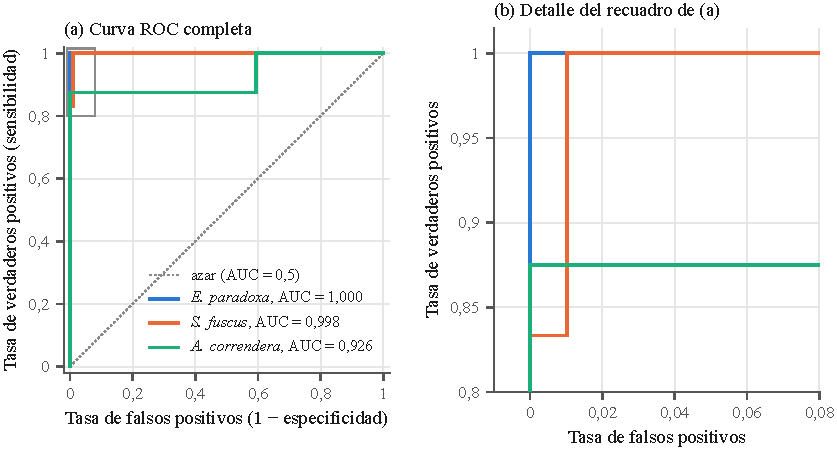
\includegraphics[width=\textwidth]{fig_roc}}{\fbox{figura pendiente}}
  \caption{Curvas ROC de la CNN de audio (prueba, protocolo agregado) para
  tres especies con al menos seis grabaciones de prueba: una con AUC igual
  a uno (\textit{Eugralla paradoxa}), la mediana (\textit{Scytalopus
  fuscus}, 0,998) y la de menor AUC (\textit{Anthus correndera}, 0,926). La
  diagonal es el clasificador al azar; el panel (b) amplía el recuadro de
  (a).}
  \label{fig:roc}
\end{figure}

En el modelo de distribución el AUC es la métrica estándar
\citep{valavi2022benchmark}: para cada especie compara las probabilidades
asignadas a las presencias de prueba con las de los puntos de fondo. Hay dos
salvedades. Como los puntos de fondo no son ausencias reales, el AUC mide la
capacidad de distinguir presencias del ambiente disponible, no de ausencias
verdaderas, y sus valores son relativos: solo permiten comparar modelos de
una misma especie en una misma área \citep[p.~265]{guisan2017hsdm}. Además,
es poco sensible al tamaño muestral y a la prevalencia, lo que lo vuelve
optimista \citep[p.~120]{guisan2017hsdm}, y depende de la extensión del
área de estudio \citep{lobo2008auc}. Por eso la tesis lo usa para comparar
métodos sobre los mismos datos, no como valor absoluto.

\subsection{Incertidumbre de las métricas}

Con conjuntos de prueba pequeños las métricas son ruidosas: una grabación
más o menos acertada cambia el F1 de una especie con tres muestras de 1,00 a
0,80, y dos errores lo bajan a 0,50. Esta tesis estima la incertidumbre con el \textit{bootstrap}
\citep{efron1993bootstrap}: se remuestrea el conjunto de prueba con
reemplazo $R$ veces, se recalcula la métrica en cada remuestra y los
percentiles 2,5 y 97,5 de esos valores forman el intervalo de confianza al
\SI{95}{\percent}. Para comparar dos modelos de distribución, que se evalúan
sobre las mismas especies, se usa el test de Wilcoxon de rangos con signo,
que contrasta si las diferencias de AUC por especie se distribuyen
simétricamente alrededor de cero sin suponer normalidad.

%-----------------------------------------------------------------------
\section{Autocorrelación espacial y validación por bloques}\label{sec:teoria-validacion}

\begin{figure}[!htb]
  \centering
  \IfFileExists{figuras/fig_blockcv.pdf}{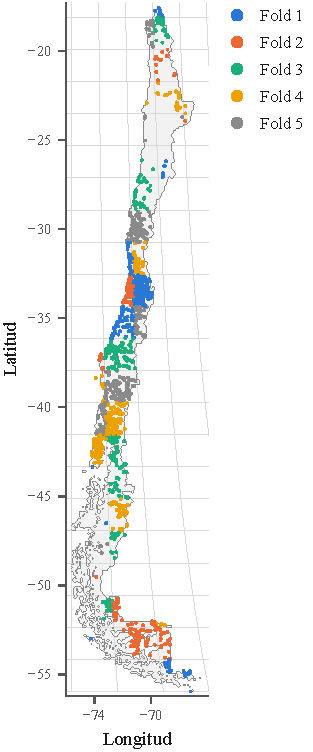
\includegraphics{fig_blockcv}}{\fbox{figura pendiente}}
  \caption{Partición espacial por bloques de \SI{200}{\kilo\metre} usada
  para validar los modelos de distribución: muestra de 8\,000 de los
  34\,926 puntos del conjunto del SDM, coloreados según el \textit{fold} de
  su bloque (46 bloques repartidos al azar en cinco \textit{folds} de tamaño
  equilibrado). Cada \textit{fold} de prueba contiene bloques completos
  ausentes del entrenamiento.}
  \label{fig:blockcv}
\end{figure}

La \figref{fig:blockcv} muestra la partición espacial que usa esta tesis;
esta sección explica por qué hace falta. Los datos ecológicos violan un
supuesto básico de la evaluación: las
observaciones cercanas no son independientes, porque comparten ambiente,
historia y, en ciencia ciudadana, observador. Esta \emph{autocorrelación
espacial} se mide con el semivariograma, que promedia las diferencias al
cuadrado entre pares de puntos separados por una distancia $d$:
\begin{equation}
  \gamma(d) = \frac{1}{2\,|N(d)|} \sum_{(i,j) \in N(d)} \big(z_i - z_j\big)^2,
  \label{eq:variograma}
\end{equation}
donde $N(d)$ son los pares a distancia aproximadamente $d$ y $z$ una
covariable. La \figref{fig:semivariograma} muestra su forma típica: la
semivarianza crece con la distancia hasta estabilizarse en la \emph{meseta},
el valor que corresponde a dos puntos sin relación entre sí; el
\emph{rango} es la distancia a la que se alcanza esa meseta, a partir de la
cual dos puntos ya no se parecen más que dos puntos cualesquiera; y el
\emph{efecto pepita} es la semivarianza en el origen, que recoge el ruido
de medición y la variación a escalas menores que la distancia mínima entre
puntos.

\begin{figure}[!htb]
  \centering
  \IfFileExists{figuras/fig_semivariograma.pdf}{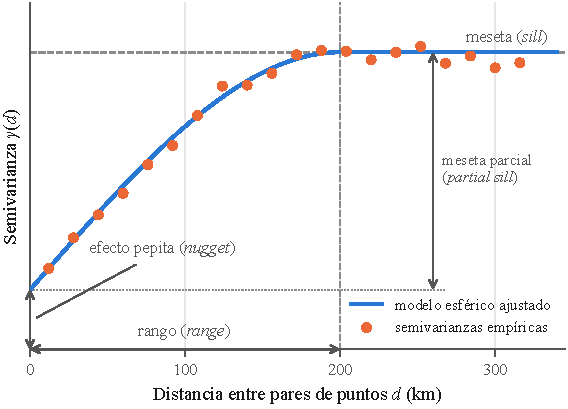
\includegraphics[width=0.66\textwidth]{fig_semivariograma}}{\fbox{figura pendiente}}
  \caption{Semivariograma esquemático: semivarianzas empíricas por clase de
  distancia y modelo esférico ajustado, con sus tres parámetros: efecto
  pepita (valor en el origen), meseta (valor estable) y rango (distancia a
  la que se alcanza la meseta), que aquí fija el tamaño de los bloques de
  validación.}
  \label{fig:semivariograma}
\end{figure}
 Si entrenamiento y prueba se reparten al azar, cada punto de
prueba tiene vecinos casi idénticos en entrenamiento y las métricas resultan
infladas \citep[pp.~276, 297]{guisan2017hsdm}. En audio el consejo es el
mismo: nunca repartir grabaciones de un mismo lugar o archivo entre
entrenamiento y prueba \citep[pp.~161, 166]{virtanen2018casse}. La
validación cruzada por bloques \citep{roberts2017crossvalidation,
valavi2019blockcv} divide el territorio en bloques contiguos de tamaño
comparable al rango de autocorrelación, asigna los bloques al azar a cinco
\textit{folds} y evalúa cada modelo en bloques que nunca vio. Mide, por
tanto, la capacidad de
\emph{extrapolar} a zonas sin registros, que es más exigente que la de
interpolar entre registros vecinos (\figref{fig:blockcv}). Ambos protocolos
se reportan en el \capref{cap:resultados}.


%-----------------------------------------------------------------------
\section{Metodología de trabajo, fuentes de datos y \textit{baselines}}
\label{sec:herramientas}

\subsection{Metodología de trabajo}

El proyecto se organiza según la metodología CRISP-DM: comprensión del
problema, comprensión y preparación de los datos (\capref{cap:datos}),
modelado, evaluación y despliegue (\capref{cap:resultados}), fases recorridas de
forma iterativa. Todo el desarrollo se realiza en Python con PyTorch
\citep{paszke2019pytorch}, sobre
un repositorio versionado cuyas dependencias se gestionan con \texttt{uv}
para garantizar la reproducibilidad de los experimentos.

\subsection{Fuentes de datos}

La \tabref{tab:fuentes} resume las fuentes públicas integradas, su
modalidad, cobertura y uso en el proyecto. MODIS es el sensor de los
satélites Terra y Aqua de la NASA del que proviene el NDVI. Google Earth
Engine (GEE) no es una fuente de datos, sino la plataforma en la nube desde
la que se consultan MODIS, WorldClim y SRTM sin descargar las imágenes
completas (\secref{sec:covariables}).

\begin{table}[!htb]
  \centering\footnotesize
  \caption{Fuentes de datos integradas en el proyecto. El plan original
  contemplaba ERA5 \citep{hersbach2020era5} y Sentinel-2
  \citep{drusch2012sentinel2}; su reemplazo se explica en el
  \capref{cap:datos}.}
  \label{tab:fuentes}
  \begin{tabularx}{\textwidth}{@{}>{\raggedright\arraybackslash\hsize=1.2\hsize}X l l l >{\raggedright\arraybackslash\hsize=0.8\hsize}X@{}}
    \toprule
    Fuente & Modalidad & Cobertura & Licencia & Uso en el proyecto \\
    \midrule
    Xeno-canto \citep{vellinga2015xenocanto} & Audio & Global & CC (varias) & Grabaciones etiquetadas por especie focal \\
    iNaturalist / GBIF \citep{vanhorn2018inaturalist} & Imagen & Global & CC (varias) & Fotografías geolocalizadas con grado de investigación \\
    eBird e iNaturalist vía GBIF \citep{sullivan2014ebird} & Tabular & Global & Abierta (CC) & Registros de presencia georreferenciados con fecha \\
    MODIS vía GEE \citep{didan2021mod13a2, gorelick2017gee} & Satelital & Global, \SI{1}{\kilo\metre} & Abierta & NDVI por punto y año \\
    WorldClim y SRTM vía GEE \citep{hijmans2005worldclim, farr2007srtm} & Climática, topográfica & Global, \SI{1}{\kilo\metre} & Abierta & Temperatura, precipitación y elevación \\
    RCE -- MMA \citep{mma2026rce} & Documental & Chile & Pública & Categoría de conservación; selección de especies \\
    \bottomrule
  \end{tabularx}
\end{table}

\subsection{Selección de \textit{baselines}}

Los \textit{baselines} se eligieron pensando en dos dimensiones: cómo se
abordaría cada problema \emph{hoy, sin este proyecto}, y cómo se abordaría
\emph{con un método más antiguo o más simple}. La \tabref{tab:baselines-def}
los organiza por tarea y resume la configuración de cada uno. Los
hiperparámetros completos están en el Apéndice~\ref{ape:hiperparametros}.

\begin{table}[!htb]
  \centering\footnotesize
  \caption{\textit{Baselines} del proyecto, por tarea y por dimensión de
  comparación.}
  \label{tab:baselines-def}
  \begin{tabularx}{\textwidth}{@{}>{\raggedright\arraybackslash\hsize=0.55\hsize}X >{\raggedright\arraybackslash\hsize=1.25\hsize}X >{\raggedright\arraybackslash\hsize=1.2\hsize}X@{}}
    \toprule
    Tarea & Práctica actual (sin este proyecto) & Método más simple o más antiguo \\
    \midrule
    Identificación de especies &
    (i) Clasificadores unimodales (solo audio o solo imagen), la forma
    habitual de identificación automática: los mismos modelos de esta tesis
    evaluados sin fusión.
    (ii) Un modelo de IA generativa multimodal (Claude Opus 5.5) consultado
    con la fotografía y la lista de especies candidatas, en
    \textit{zero-shot} y \textit{few-shot} (una fotografía de referencia por
    especie); temperatura por defecto (1,0), esfuerzo de razonamiento bajo,
    salida estructurada restringida a la lista. &
    Regresión logística sobre los \textit{frozen embeddings} de los mismos
    modelos preentrenados sin ajustar (EfficientNet-B0 y B3 de ImageNet,
    AST de AudioSet), siguiendo a \citet{ghani2023embeddings}: mide cuánto
    aporta el ajuste completo. \\
    \midrule
    Distribución de especies &
    MaxEnt, el método de referencia en ecología, implementado como regresión
    logística penalizada (L2, $C = 1$) con \textit{features} lineales y
    cuadráticas (Ecuación~\ref{eq:logistica}). &
    El propio MaxEnt es también el método clásico; frente a él se comparan
    Random Forest ($B = 300$), gradient boosting ($J = 300$, $\nu = 0{,}05$)
    y la red neuronal conjunta (Ecuación~\ref{eq:deepsdm}). \\
    \bottomrule
  \end{tabularx}
\end{table}

%-----------------------------------------------------------------------
\section{Justificación técnica de la metodología}\label{sec:justificacion}

\textbf{Transfer learning.} El conjunto de datos chileno es pequeño
(\num{2508} grabaciones de 55 especies y \num{7060} fotografías de 53), lo que
hace inviable entrenar redes profundas desde cero. Los modelos preentrenados
en ImageNet y AudioSet reutilizan representaciones aprendidas sobre millones
de ejemplos y solo necesitan ajustarse a la nueva tarea
(\secref{sec:teoria-transfer}). Que los \textit{embeddings} de clasificadores
de aves transfieran incluso con pocos ejemplos por clase
\citep{ghani2023embeddings} es valioso para las especies amenazadas, que son
las que menos datos tienen.

\textbf{Late fusion.} Aporta robustez frente a registros ambiguos o
incompletos: un canto grabado con ruido puede complementarse con una
fotografía y viceversa. Permite entrenar cada rama con datos no
emparejados, que es la situación de Xeno-canto e iNaturalist, donde audio e
imagen de un mismo individuo raramente coexisten, y opera cuando solo hay
una modalidad (\secref{sec:teoria-fusion}). Los resultados de SSW60
muestran que esta combinación mejora el desempeño sobre cada modalidad por
separado \citep{vanhorn2022ssw60}.

\textbf{Balanceo y aumentación.} La pérdida ponderada por clase, SpecAugment
y \textit{mixup} (\secref{sec:teoria-regularizacion}) abordan el desbalance
y la escasez propios de los datos de ciencia ciudadana. Sin ellas, el
clasificador se sesgaría hacia las especies comunes en desmedro de las
amenazadas y memorizaría un corpus de pocas decenas de grabaciones por
especie.

\textbf{Covariables ambientales.} Google Earth Engine muestrea las
covariables en la nube sobre todo el territorio continental y evita
descargar y almacenar volúmenes masivos de imágenes satelitales
\citep{gorelick2017gee}. Las climatologías grilladas de WorldClim son el
conjunto de datos climáticos más usado en ecología y ofrecen cobertura
nacional homogénea, más práctica a escala que las estaciones
meteorológicas, cuya distribución en Chile es irregular
\citep[p.~63]{guisan2017hsdm}.

\textbf{Modelado de distribución.} La red conjunta multiespecie comparte
información estadística entre especies con distribuciones similares, lo que
beneficia a las de pocos registros. Los ensambles de árboles aportan una
referencia fuerte y robusta en datos tabulares
\citep{valavi2022benchmark}, y MaxEnt, como regresión logística, aporta
interpretabilidad. La validación espacial por bloques
(\secref{sec:teoria-validacion}) permite comprobar que la comparación no
esté inflada por autocorrelación.

\textbf{Baselines exigentes.} Elegir MaxEnt, un modelo de IA generativa y
los \textit{frozen embeddings} como referencias asegura que las mejoras
reportadas sean significativas en la práctica y no artefactos de una
comparación débil.

%-----------------------------------------------------------------------
\section{Efectos positivos esperados}\label{sec:efectos}

Se espera que el sistema identifique al menos 50 especies de aves chilenas
con una \textit{accuracy} superior al \SI{85}{\percent}, que la fusión
multimodal supere a los clasificadores unimodales en \textit{accuracy} y F1
macro y que el SDM basado en aprendizaje automático supere a MaxEnt en
AUC-ROC. Más allá de las métricas, los efectos positivos esperados de la
aplicación de estos elementos son:

\begin{enumerate}[label=(\roman*), leftmargin=*, itemsep=2pt]
  \item Una herramienta de apoyo al monitoreo automatizado de biodiversidad
        para organismos de conservación (MMA, CONAF, SAG) y ONG (ROC,
        CODEFF), alineada con las líneas de acción de investigación y
        monitoreo de la Estrategia Nacional de Conservación de Aves
        \citep{mma2022enca}.
  \item Un insumo para la ciencia ciudadana y la identificación asistida de
        aves, que puede retroalimentar la calidad de los registros en
        plataformas como eBird e iNaturalist.
  \item Mapas de probabilidad de presencia que permitan priorizar zonas de
        monitoreo y evaluar el efecto de variables climáticas y de vegetación
        sobre la distribución de especies amenazadas.
  \item Un repositorio reproducible que reduzca el costo de entrada para
        futuros trabajos sobre otras especies o regiones.
  \item Evidencia metodológica cuantitativa sobre la escasez de datos en
        especies amenazadas y sobre la efectividad de las estrategias de
        mitigación, útil para orientar esfuerzos de recolección de datos.
\end{enumerate}
